% Begin Preamble --------------------------------------------------------------

\documentclass[12pt,english]{article}
\usepackage{amsmath}
\usepackage{txfonts}
\usepackage[scaled=0.92]{helvet}
\usepackage{courier}
\renewcommand{\familydefault}{ptm}
\renewcommand{\rmdefault}{ptm}
\renewcommand{\sfdefault}{phv}
\renewcommand{\ttdefault}{pcr}
\usepackage{graphicx}
\usepackage{rotating}
\usepackage{longtable}
\usepackage{geometry}
\geometry{
	verbose,
	letterpaper,
	tmargin=90pt,
	bmargin=90pt,
	lmargin=90pt,
	rmargin=90pt,
	headheight=36pt,
	headsep=36pt,
	footskip=36pt
}
\usepackage{fancyhdr}
\pagestyle{fancy}
\usepackage[dvipsnames]{xcolor}
\usepackage{array}
\usepackage{varioref}
\setlength{\parskip}{\medskipamount}
\setlength{\parindent}{0pt}

\newcommand{\lyxline}[1][1pt]{%
  \par\noindent%
  \rule[.5ex]{\linewidth}{#1}\par}

\usepackage{lastpage}
\fancyhead{}
\lhead{\small{  \textsl{TBRS Digital Receiver Simulation} } }
\rhead{\footnotesize{  \textsl{ \today } } }
\rfoot{ \it Page \rm \thepage\   \it of \ \rm \pageref{LastPage}   }
\renewcommand{\headrulewidth}{1.0pt}
\renewcommand{\footrulewidth}{1.0pt}
\cfoot{}

\usepackage[pdftex,
            pagebackref=true,
            colorlinks=true,
            linkcolor=darkgray,
            pdfview=Fit,
            pdfpagemode=UseThumbs,
            unicode
           ]{hyperref}

\usepackage{babel}

\newcommand{\lp}{\left(}
\newcommand{\rp}{\right)}
\newcommand{\ls}{\left[}
\newcommand{\rs}{\right]}
\newcommand{\lb}{\left\{}
\newcommand{\rb}{\right\}}

% End Preamble ----------------------------------------------------------------



\begin{document}



% Begin Title Page ------------------------------------------------------------
\newpage{}

% Report Title
\title{Ten Beam Receiver Subsystem (TBRS)\\
Digital Receiver (DR) Simulation}

% Report Author
\author{Gary Stephens\\ Son Trinh}

% Report date
\date{
\today
}

\maketitle

% Report Subtitle
\noindent \begin{center}
CONTROL AND SIGNAL PROCESSING UPGRADE (CSPU)\\
SYSTEM ENGINEERING AND SUSTAINMENT INTEGRATOR (SENSOR)\\
SUBCONTRACT NO. 40316, CLIN 0318
\par\end{center}


% Report Recipient
\noindent \begin{center}
Prepared for:\\
\medskip{}
SENSOR\\
ITT Corporation Systems Division\\
4450 East Fountain Boulevard\\
Colorado Springs, CO 80916-2153
\par\end{center}

% Report Preparer
\noindent \begin{center}
Prepared by:\\
\medskip{}
Technology Service Corporation\\
Phase IV Systems Operation\\
3405 Triana Boulevard\\
Huntsville, AL 35805-4695
\par\end{center}

\thispagestyle{empty}\newpage{}

% End Title Page --------------------------------------------------------------


\tableofcontents{}

\listoffigures

\listoftables

\newpage{}


\section{Introduction}\label{sec:secIntro}

This report documents the simulation of the digital receiver (DR) of
the ten-beam receiver subsystem (TBRS). This includes simulation of
the TBRS intermediate frequency (IF) analog-to-digital converter (A/D)
samples and simulatiuon of the processing of these samples.

Two separate software simulations were created. The first simulates
the IF signal samples. The second simulates the digital down
conversion (DDC) processing of the IF samples. Two simulations were
generated since the simulated IF samples are generated with pseudo
random noise (PRN) samples plus determistic signal samples. The
simulated IF signal plus noise samples are output to data files that
can be processed multiple times. This allows the same IF samples to be
processed by both the processing simulation and the actual firmware in
the TBRS. This also allows the same IF samples to be processed
multiple times as the firmware and simulation software are developed
and tested.

\subsection{Document Overview}

This document contains the following sections:
\begin{itemize}

\item This section provides an introduction.

\item Section~\vref{sec:secNBVM} describes the simulation of the IF
signal plus noise samples. This section also describes how to run the
simulation and generate IF samples.

\item Section~\vref{sec:tbrsDDC} describes the simulation of the TBRS
DDC and how to run the simulation.

\end{itemize}


% \pagebreak{}
\subsection{Abbreviations}

The following abbreviations and terms are used in this document.
\begin{description}
\item [{A/D}] Analog-to-digital converter.
\item [{BPF}] Bandpass filter.
\item [{CSPU}] Control and signal processor upgrade project.
\item [{DDC}] Digital down conversion.
\item [{DLPF}] Digital low pass filter.
\item [{DSPS}] Digital signal processing subsystem.
\item [{FIR}] Finite impulse response.
\item [{FFT}] Fast Fourier transform.
\item [{GCW}] Gated continuous wave.
\item [{HP~and~VP}] Horizontal and vertical polarization.
\item [{I~and~Q}] In-phase and quadrature-phase.
\item [{IF}] Intermediate frequency.
\item [{LFM}] Linear frequency modulation.
\item [{LPF}] Low pass filter.
\item [{LO}] Local oscillator.
\item [{MF}] Matched filter.
\item [{MP}] Multipulse.
\item [{PRN}] Pseudo-random number.
\item [{PSD}] Power spectral density.
\item [{QD}] Quadrature demodulator.
\item [{Radar}] The Eglin AN/FPS-85 phased array Radar.
\item [{SNR}] Signal-to-noise ratio.
\item [{SP}] Single pulse.
\item [{Specification}] DSPS specification.
\item [{TBRS}] Ten-beam receiver subsystem.
\item [{VM}] Vector modulator.
\item [{WSS}] Wide sense stationary.
\end{description}

\clearpage
\pagebreak{}
\section{Simulation of TBRS IF A/D Samples}\label{sec:secNBVM}

This section describes the simulation of the TBRS IF A/D samples.

\subsection{Simulation Overview}

The analog inputs to the TBRS contain two narrowband (bandpass) signal
plus noise components multiplexed in frequency. These are the
horizontal polarization (HP) and vertical polarization (VP) returns
from a radar target. Both components have a bandwidth of approximately
1 MHz. The HP component is centered at 20.5 MHz and extends from 20 to
21 MHz. The VP component is centered at 23.5 MHz and extends from 23
to 24 MHz. The overall HP/VP spectrum is centered at 22 MHz.

The TBRS samples each analog input with a 14-bit A/D at a 60 MHz
sampling rate. Two software vector modulators (VM) are used to
simulate the HP and VP bandpass signal plus noise components.  A block
diagram of the HP modulator is shown in Figure~\vref{fig:VectorModulator}.
The VP modulator is identical except for the parameters.

\begin{figure}[htbp]
  \noindent \begin{centering}
  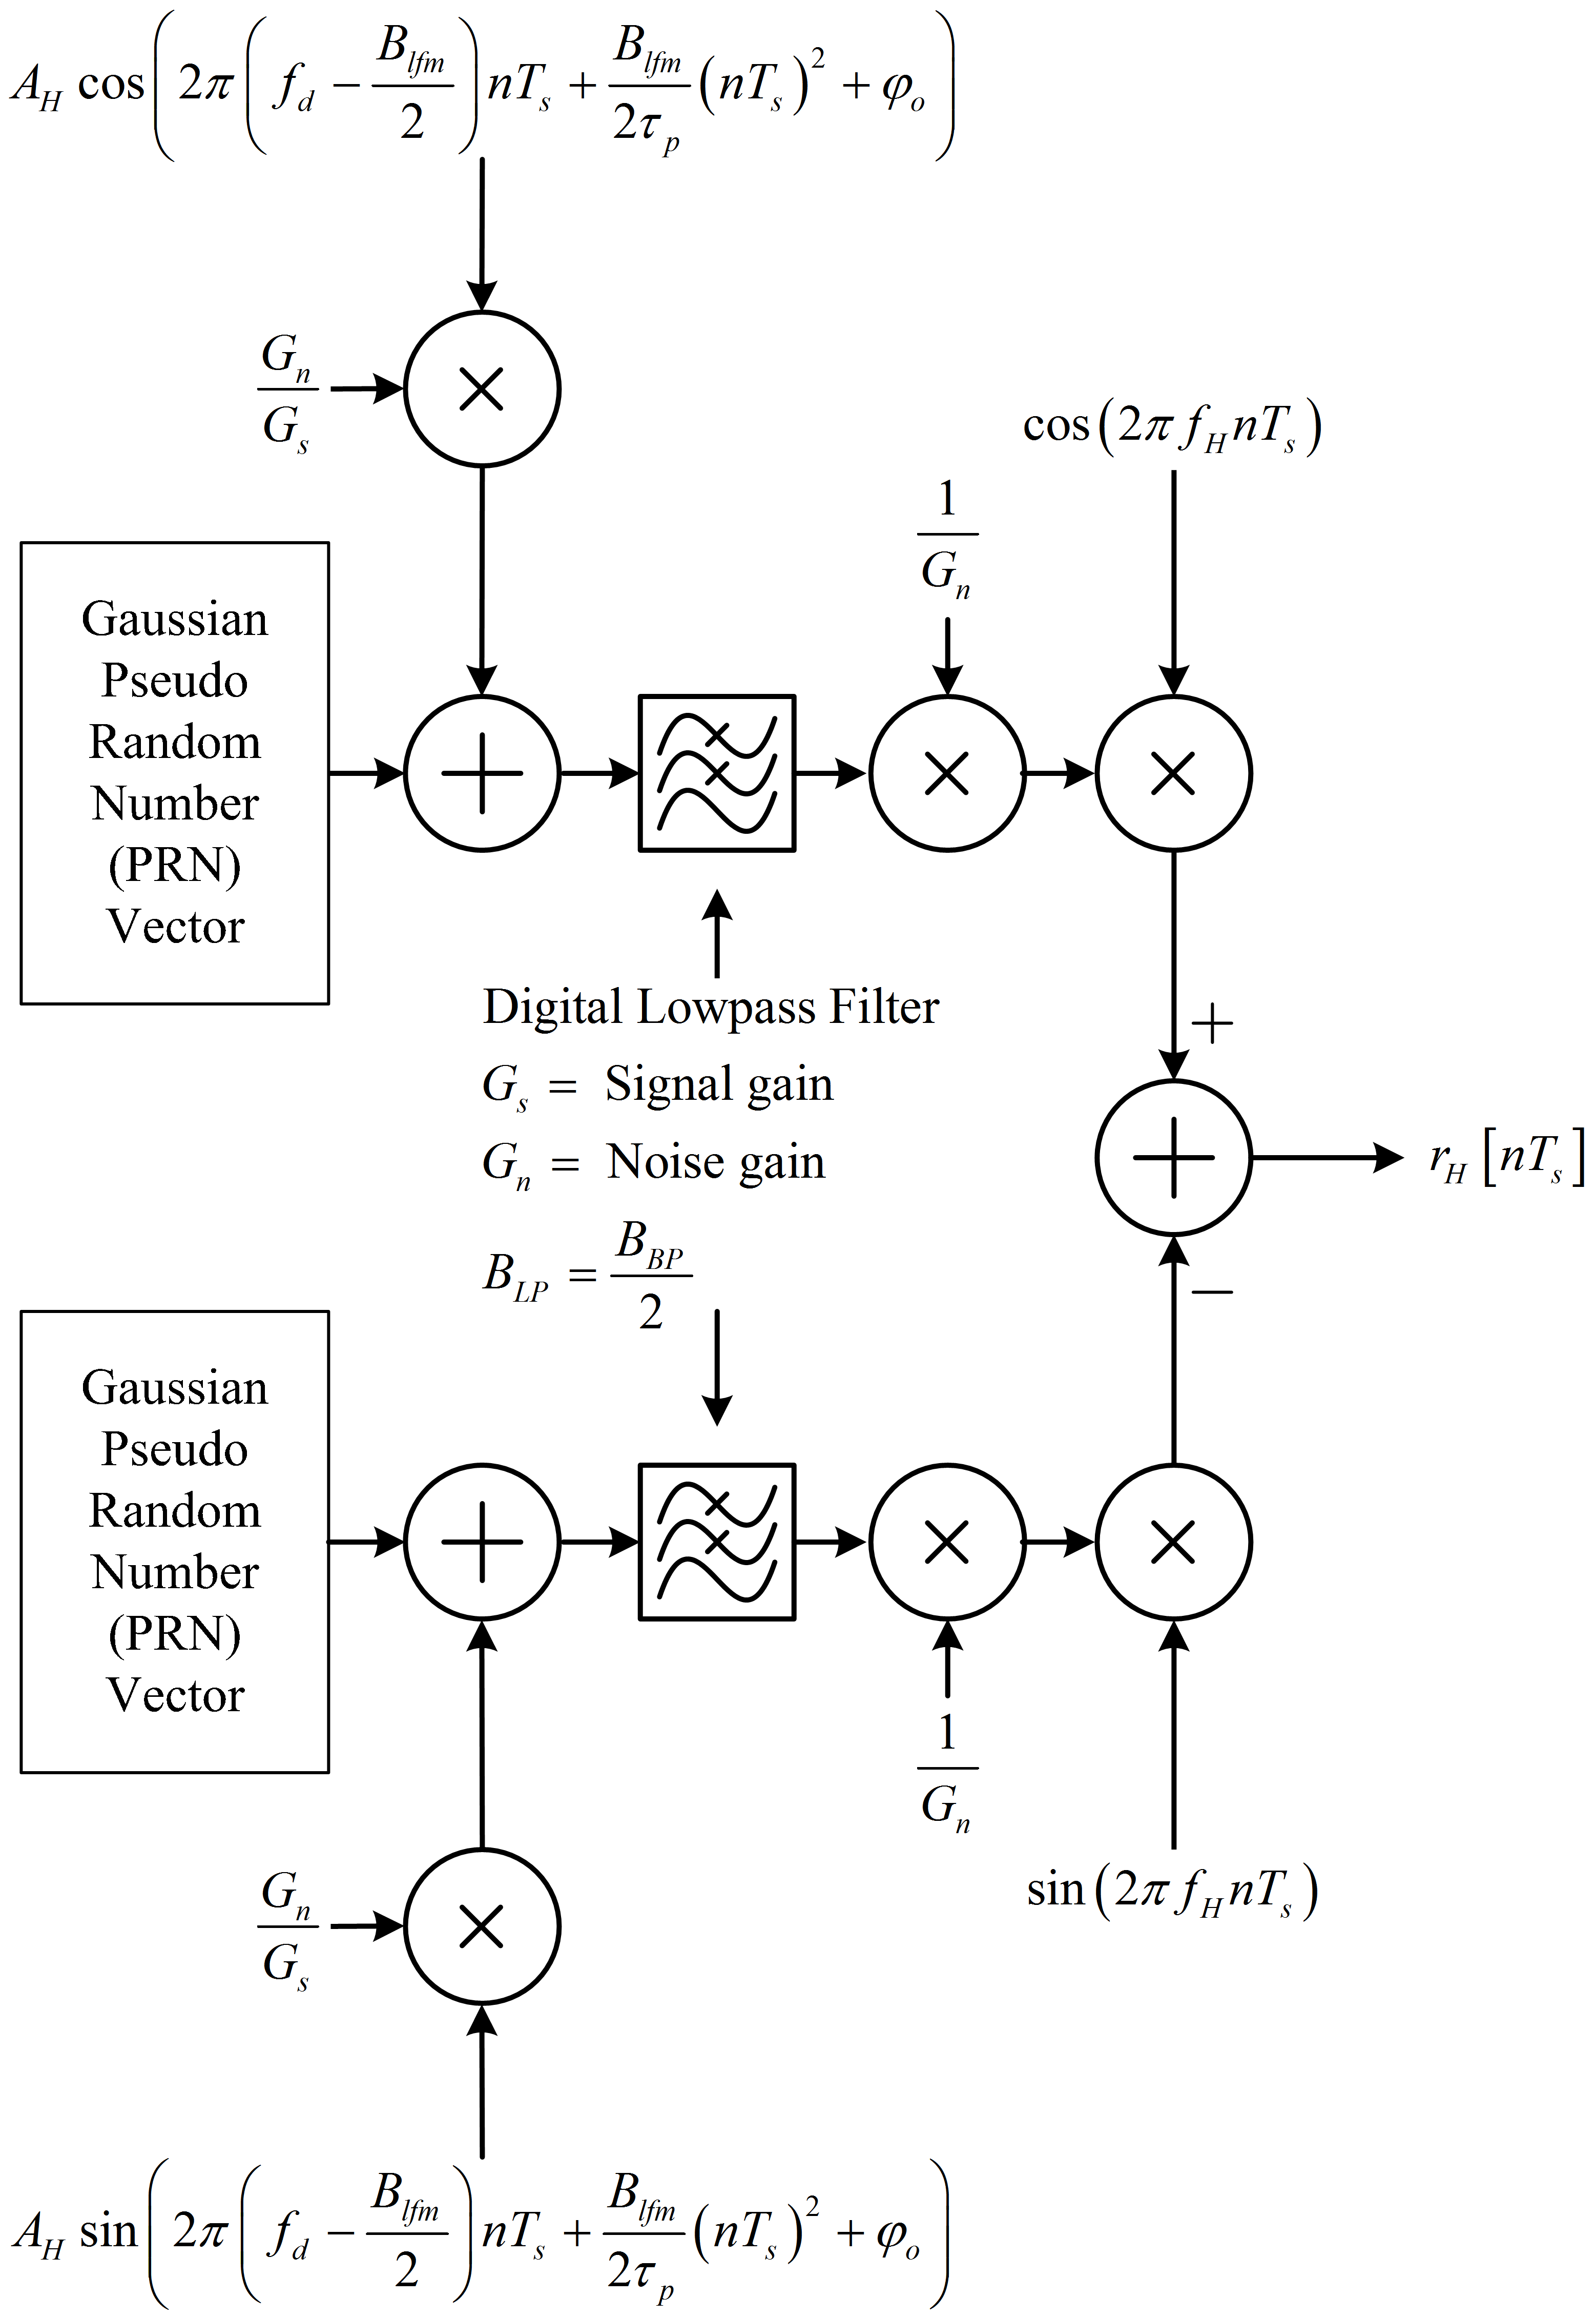
\includegraphics{VectorModulator.png}\medskip{}
  \caption{Digital Vector Modulator}
  \label{fig:VectorModulator}
  \par \end{centering}
\end{figure}

A software Gaussian pseudo-random number (PRN) generator is used to
generate the two independent, zero mean, white Gaussian noise vectors
shown in the figure. The standard deviation $\sigma$ of the noise
samples in counts is calculated from the analog bandpass noise power
in dBm input to the simulation.

The noise samples are added to baseband quadrature signal samples.
These are the baseband in-phase and quadrature-phase (I~and~Q)
components of the CSPU waveforms sampled at the TBRS A/D sampling rate
$f_s = 60$ MHz. The sampling period $T_s$ is the the inverse of the
sampling frequency. This includes both linear frequency modulated
(LFM) and gated continuous wave (GCW) signals. The LFM bandwidth is
$B_{lfm}$ and is zero for GCW waveforms.  The pulse width is $\tau_p$
and the amplitude in counts is $A_H$ for the HP modulator. The
amplitude in counts is calculated from the signal power level in dBm
input to the simulation.

The signal amplitude is scaled prior to the addition. This will be
explained shortly. The combined signal plus noise samples are lowpass
filtered with digital lowpass filters (DLPF) to set the noise
bandwidth. This also limits the signal bandwidth. The DLPF has a noise
gain of $G_n$ and a signal gain of $G_s$. The output of the filter is
scaled by $1/G_n$ so that the standard deviation of noise at the
filter output is equal to the desired value $\sigma$. The signal gain
through the filter is $G_s$, so the signal is pre-scaled by $G_n/G_s$
so that the signal amplitude at the filter output is~$A_H$.

The DLPF is a finite impulse response (FIR) filter with $N$ impulse
response samples $w_i$. The signal and noise gain through the filter
are given as
\begin{eqnarray*}\label{eq:firSignalNoiseGain}
  G_s &=& \sum_{i=0}^{N-1} w_i \\
  G_n &=& \sqrt{\sum_{i=0}^{N-1} w^2_i}
\end{eqnarray*}
This assumes that the input noise samples are independent and the
noise spectrum is white.

The filter outputs are scaled and then modulated to the center
frequency $f_H$. This converts the I and Q lowpass signal plus noise
samples to bandpass signal plus noise processes at the desired center
frequency and sampling rate. The resulting banpass samples are called
$r_H \ls n T_s \rs$

The composite HP and VP bandpass signal plus noise samples are
simulated with two software VM objects as shown in
Figure~\vref{fig:TbrsDualVM}.  The signal amplitudes $A_H$ and
$A_V$, and noise standard deviations $\sigma_H$ and $\sigma_V$ of each
VM are set independently, though the noise standard deviations are
typically set equal. The quadrature LO frequencies are $f_H = 20.5$
and $f_V = 23.5$ MHz. The pulse width and LFM bandwidth are set by the
CSPU waveform being simulated and are common to both VMs. The 11 CSPU
waveforms are listed in Table~\vref{tab:cspuWfms}

\begin{table}[ht]
  \noindent \begin{centering}
  \caption{CSPU Waveforms}
  \medskip{}
  \label{tab:cspuWfms}
  \begin{tabular}{|l|l|l|}
  \hline
  Pulse Type  & $\tau_p$ (usec.) & $B_{lfm}$ (MHz) \\ \hline
  1           &  1               &  0          \\ \hline
  2           &  10              &  0          \\ \hline
  3           &  16              &  1          \\ \hline
  4           &  25              &  0          \\ \hline
  5           &  32              &  1          \\ \hline
  6           &  64              &  1          \\ \hline
  7           &  125             &  0          \\ \hline
  8           &  128             &  0.1        \\ \hline
  9           &  128             &  1          \\ \hline
  10          &  250             &  0.1        \\ \hline
  11          &  250             &  1          \\ \hline
  \end{tabular}
  \par \end{centering}
\end{table}

The outputs the vector modulators ($r_H \ls n T_s \rs$ and $r_V \ls n
T_s \rs$) are summed and a constant $\mu$ is added to simulate the
unwanted DC offset of the A/D. The processing up to this point is
performed in floating point. The floating point samples are rounded to
simulate the TBRS A/D quantization. The resulting samples are called
$r \ls n T_s \rs$.

\begin{figure}[htbp]
  \noindent \begin{centering}
  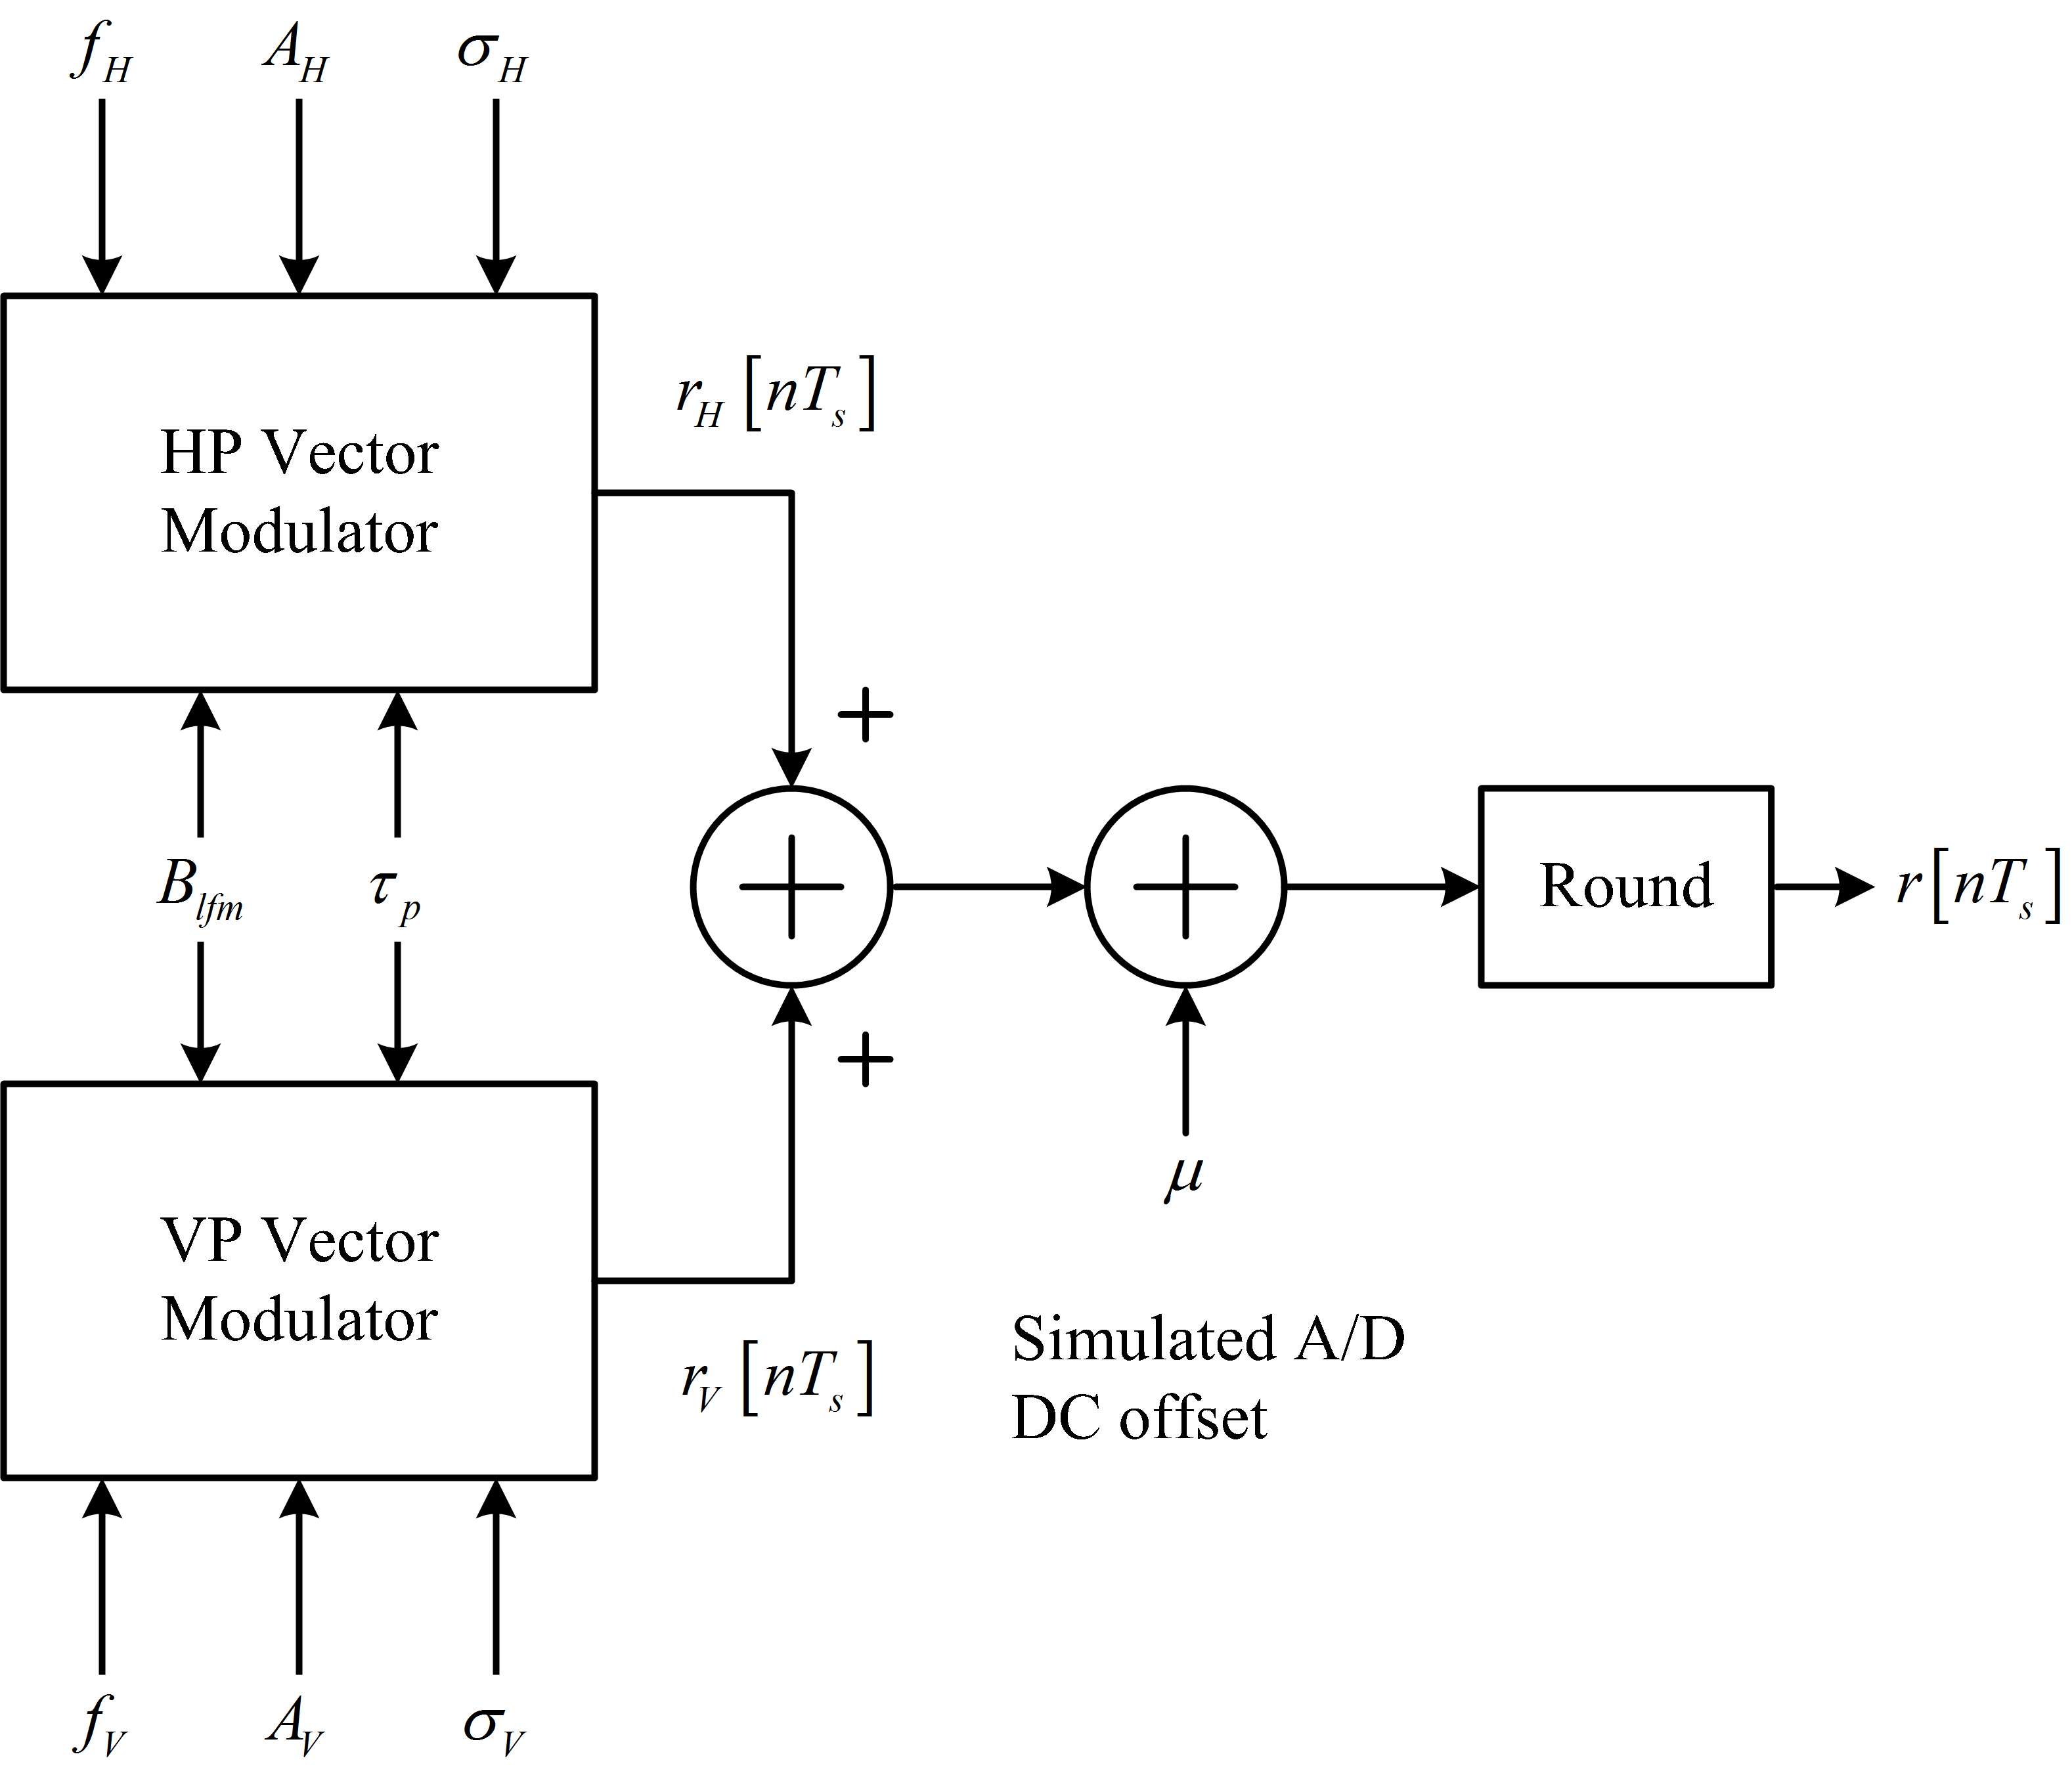
\includegraphics[width=5.0in]{TbrsDualVM.png}\medskip{}
  \caption{Dual Vector Modulators}
  \label{fig:TbrsDualVM}
  \par \end{centering}
\end{figure}

\subsection{Calculation of Signal and Noise Count Values}

The TBRS A/D characteristics and the typical A/D input noise level
must be considered to properly simulate the A/D output samples. The
TBRS A/D is a 14-bit device. The output numeric format is two's
complement, so the range is from $-2^{13}$ to~$+2^{13}-1$. The A/D
reaches full scale output when the input is at~+10~dBm into 50~ohms.
Solving for the input full scale voltage gives
\begin{eqnarray}
  10 \log_{10} \lp \frac{A_{fs}^2}{2R} \rp + 30 &=& +10 \\
  \log_{10} \lp \frac{A_{fs}^2}{100} \rp &=& -2 \nonumber\\
  \frac{A_{fs}^2}{100} &=& 10^{-2} \nonumber\\
  A_{fs}^2 &=& 1 \nonumber\\
  A_{fs} &=& 1 \mbox{ volt.} \nonumber
\end{eqnarray}

The shows that the full scale input is 1 volt. The voltage
quantization is
\begin{equation}
  v_q = \frac{1}{8192} = 122.07 \times 10^{-6} \mbox{ volts.}
\end{equation}

The noise level into the A/D is nominally set so that the noise standard
deviation in counts will be $\sigma = 3 v_q$. This gives a noise power of
\begin{eqnarray}\label{eq:noise3q}
  P_n &=&  10 \log_{10} \lp \frac{\sigma^2}{R} \rp + 30 \\
      &=&  10 \log_{10} \lp \frac{134.11 \times 10^{-9}}{50} \rp + 30 \nonumber\\
      &=&  -85.72 + 30 \nonumber\\
      &=&  -55.72 \mbox{ dBm.} \nonumber
\end{eqnarray}

The HP and VP peak signal power and noise power in dBm are input to
the simulation. These values must be converted to counts when
generating the inputs to the dual VMs. The peak signal level in volts
and counts is given as
\begin{eqnarray}\label{eq:amplitudeCounts}
  P_s &=& 10 \log_{10} \lp \frac{A_v^2}{2R} \rp + 30 \nonumber\\
  10^{ \frac{P_s - 30}{10}} &=& \frac{A_v^2}{100} \nonumber\\
  A_v &=& 100 \cdot 10^{ \frac{P_s - 30}{20}} \nonumber\\
    &=& 10^{1 + \frac{P_s - 30}{20}} \nonumber\\
  A_c &=& \frac{A_v}{v_q}.
\end{eqnarray}

The nominal noise power is given by equation~\vref{eq:noise3q} and the
noise standard deviation in counts is~3 . If a lower or higher noise
power is desired, the conversion from power in dBm to noise standard
deviation in volts and counts is given as
\begin{eqnarray}\label{eq:noiseCounts}
  P_n &=& 10 \log_{10} \lp \frac{\sigma_v^2}{R} \rp + 30 \nonumber\\
  10^{ \frac{P_n - 30}{10}}  &=& \frac{\sigma_v^2}{50} \nonumber\\
  \sigma_v &=& \sqrt{50} \cdot 10^{ \frac{P_n - 30}{20}} \nonumber\\
  \sigma_c &=& \frac{\sigma_v}{v_q}.
\end{eqnarray}

The amplitude and noise counts set in the equations above are for both
the HP and VP narrowband processes. If the noise power is set to
-55.72 dBm for both HP and VP, then each will have -55.72 dBm.

\subsection{Executing the Simulation}

The simulation was generated using the open source Python programming
language with additional open source scientific and graphics
libraries. This includes the following:
\begin{itemize}

\item Python version 2.5.4. This is the core Python language.

\item NumPy multi-dimensional array library version 1.3.0.

\item Matplotlib plotting library version 0.99.0.

\item wxPython graphical user interface library version 2.8.10.1.

\item SciPy advanced math and signal processing library version 0.7.1.

\end{itemize}
These items can all be obtained separately, but it is much easier to
install Python and the required libraries using the integrated
installer available at www.pythonxy.com. This site maintains the
required packages and libraries and includes a ``one-click'' installer
for the Windows platform.

The IF simulation main source file is named \texttt{TbrsIfSim.py}.
Python is an interpreted language and no compilation to an executable
file is required. \texttt{TbrsIfSim.py} requires the following
additional files:
\begin{itemize}

\item \texttt{fir.py}. This file implements the FIR software objects
for the DLPFs in the VMs.

\item \texttt{util.py}. This file contains utility functions used by
\texttt{TbrsIfSim.py}.

\item \texttt{h767\_Dec48\_100.csv}. This ``comma separated value'' file
contains the impulse response samples for the DLPFs in the VMs.

\item Input parameter files for each pulse type to be simulated.

\end{itemize}
The input parameter files set the parameters used to simulate the IF
samples. An example for pulse type 3 is shown below. The input file
name is \texttt{pt03.inp}. The file name must begin with ``pt'' and
have extension ``.inp''. The input file should include all 10 values
as shown.

\scriptsize
\begin{verbatim}
pulseType          = 3            # CSPU pulse type.
beamID             = 5            # NOVEM antenna beam number (1..10)
numBasebandSamples = 250          # Number of output baseband samples to generate.
Ps_H               = 0.0          # HP peak signal power (dBm).
Ps_V               = -10.0        # VP peak signal power (dBm).
Pn_H               = -55.72       # HP noise power (dBm).
Pn_V               = -55.72       # VP noise power (dBm).
tau_d              = 0.550205775  # Target delay (fraction of 60 MHz IF sample window).
f_d                = 0.0          # Target Doppler frequency offset (Hz).
muIF               = 0.0          # Simulated A/D dc offset (counts).
\end{verbatim}
\normalsize

The simulation of the TBRS DDC processing
is named \texttt{TbrsSimDdc.py} and is discussed in
Section~\vref{sec:tbrsDDC}. Both \texttt{TbrsIfSim.py} and
\texttt{TbrsSimDdc.py} are designed to be executed from a common
folder. The simulated IF samples generated by \texttt{TbrsIfSim.py}
are stored in a sub-folder named \texttt{IFdata} and are read by
\texttt{TbrsSimDdc.py}. The sub-folder is created by
\texttt{TbrsIfSim.py} if it does not exist.

\texttt{TbrsIfSim.py} generates the IF data file name based on the
current date and time, and the pulse type. An example file name is
\texttt{IF\_Y2009M10D13H13M31S33PT03.dat}. The components of this file
name are:
\begin{itemize}

\item Year 2009.

\item Month 10 (October).

\item Day 13 (the thirteenth day of October).

\item Hour 13 (1:00 PM).

\item Minute 31.

\item Second 33.

\item Pulse type 3.

\item File extension ``.dat''.

\end{itemize}

\texttt{TbrsIfSim.py} generates a second file with the same base name,
but with file extension ``.txt''. This file repeats the ``.inp'' input
parameter file contents used to generate the IF data samples.
\texttt{TbrsSimDdc.py} reads the ``.dat'' and ``.txt'' files when
processing the data.

\texttt{TbrsIfSim.py} can be executed by double-clicking its name/icon
from Windows Explorer or by typing \texttt{TbrsIfSim.py <CR>} from a
command prompt opened to the simulation folder. The command line
method is preferred as status information is printed that will be
``lost'' if the the program is executed from its icon.

When \texttt{TbrsIfSim.py} executes it builds a list of available
input file and displays a dialog box to allow the user to select the
desired pulse type to simulate. This is shown in
Figure~\vref{fig:TbrsIfSimSC01}.  The files are named with 2-digit
pulse type numbers (i.e.  \texttt{pt03.inp} instead of
\texttt{pt3.inp}) so that the file list is sorted in the correct
order.
\begin{figure}[ht]
  \noindent \begin{centering}
  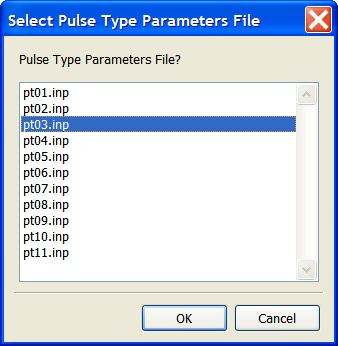
\includegraphics{TbrsIfSimSC01.png}\medskip{}
  \caption{Input Parameter File Selection Dialog}
  \label{fig:TbrsIfSimSC01}
  \par \end{centering}
\end{figure}

Next \texttt{TbrsIfSim.py} prompts the user whether to save spectral
plots as portable network graphics (.png) files as shown in in
Figure~\vref{fig:TbrsIfSimSC02}. If the user enters 1 as shown the
plot files are saved in the \texttt{IFdata} folder along with the
``.dat'' and ``.txt'' files.
\begin{figure}[ht]
  \noindent \begin{centering}
  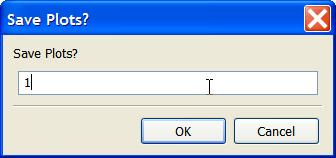
\includegraphics{TbrsIfSimSC02.png}\medskip{}
  \caption{Save Plot Files Dialog}
  \label{fig:TbrsIfSimSC02}
  \par \end{centering}
\end{figure}

The data is then generated and two spectral plots are displayed on the
screen (and optionally saved as ``.png'' files). The first plot shows
the entire 60 MHz ($\pm30$ MHz) sampled spectrum. The second plot
shows a zoom in view of the positive frequency portion of the
spectrum. The output plots for the example pulse type 3 input file are
shown in Figure~\ref{fig:IFSpectrumFull_PT3_AH2590_AV819M2} and
Figure~\vref{fig:IFSpectrumPos_PT3_AH2590_AV819M2}.

\begin{figure}[ht]
  \noindent \begin{centering}
  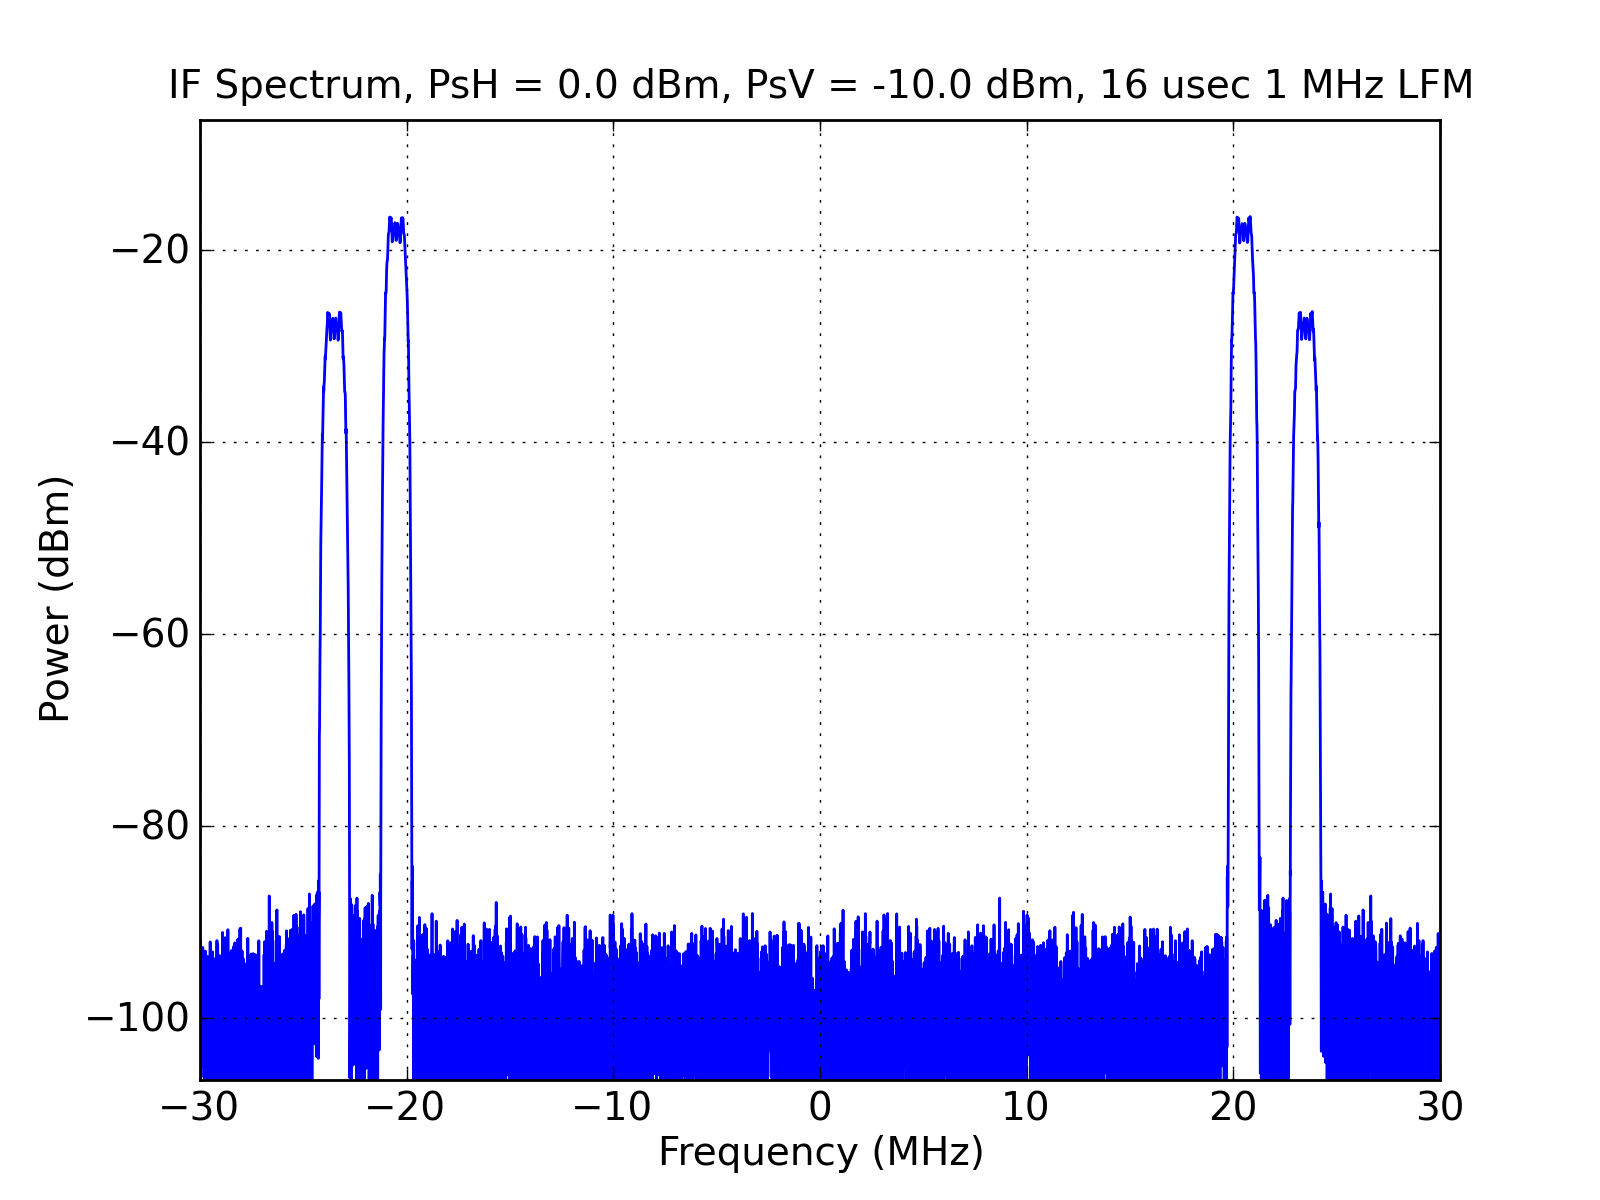
\includegraphics[width=4.75in]{IFSpectrumFull_PT3_AH2590_AV819M2.png}\medskip{}
  \caption{Full 60 MHz IF Spectrum}
  \label{fig:IFSpectrumFull_PT3_AH2590_AV819M2}
  \par \end{centering}
\end{figure}

\begin{figure}[ht]
  \noindent \begin{centering}
  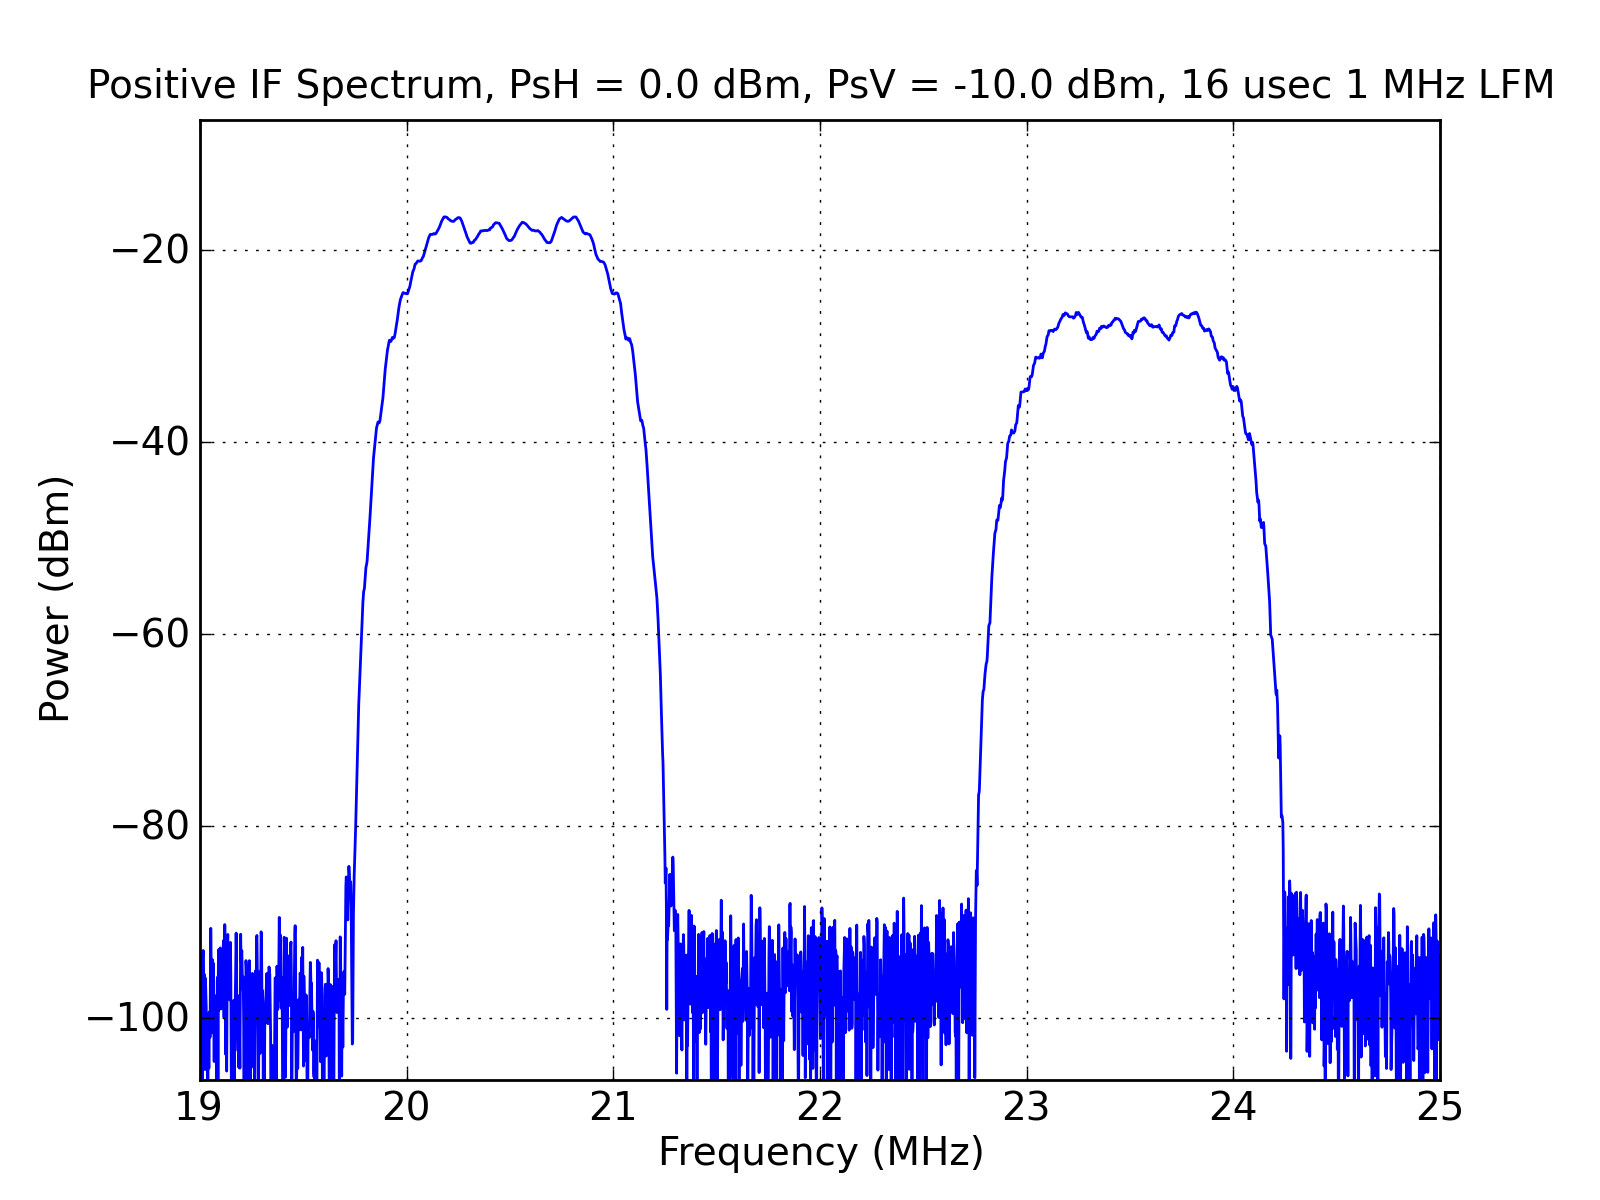
\includegraphics[width=4.75in]{IFSpectrumPos_PT3_AH2590_AV819M2.png}\medskip{}
  \caption{Zoom In View of Positive IF Spectrum}
  \label{fig:IFSpectrumPos_PT3_AH2590_AV819M2}
  \par \end{centering}
\end{figure}

Figure~\vref{fig:TbrsIfSimSC03} shows the command line execution and
the status information printed to the command prompt. This status
information is ``lost'' if \texttt{TbrsIfSim.py} is executed by
double-clicking its name/icon.
\begin{figure}[ht]
  \noindent \begin{centering}
  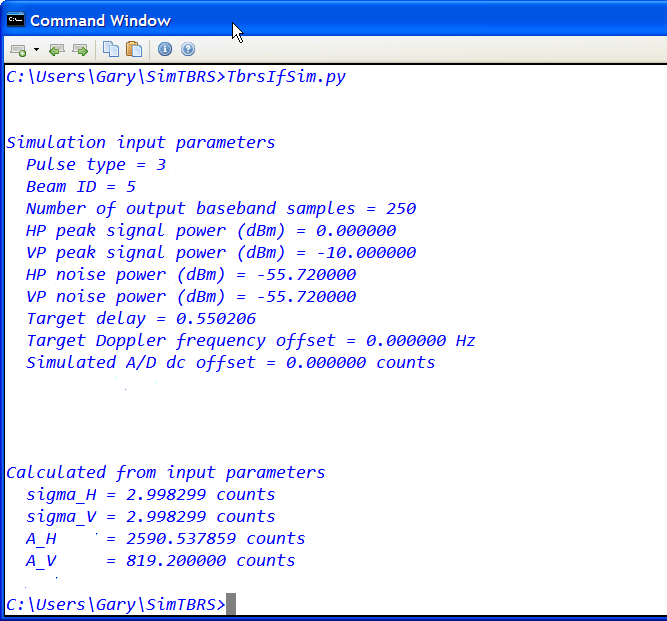
\includegraphics{TbrsIfSimSC03.png}\medskip{}
  \caption{Command Line Execution and Status}
  \label{fig:TbrsIfSimSC03}
  \par \end{centering}
\end{figure}

\clearpage
\newpage{}
\section{Simulation of the TBRS Digital Down Conversion}\label{sec:tbrsDDC}

This section describes the simulation of the TBRS DDC processing.

\subsection{Simulation Overview}

The TBRS digital down conversion (DDC) includes dual DDC circuits for
the HP and VP signal components. A top-level block diagram of the TBRS
DDC is shown in Figure~\vref{fig:TbrsDdcTopLevel}. The operation of
the DDCs is identical and will be described for the HP DDC.

\begin{sidewaysfigure}
  \noindent \begin{centering}
  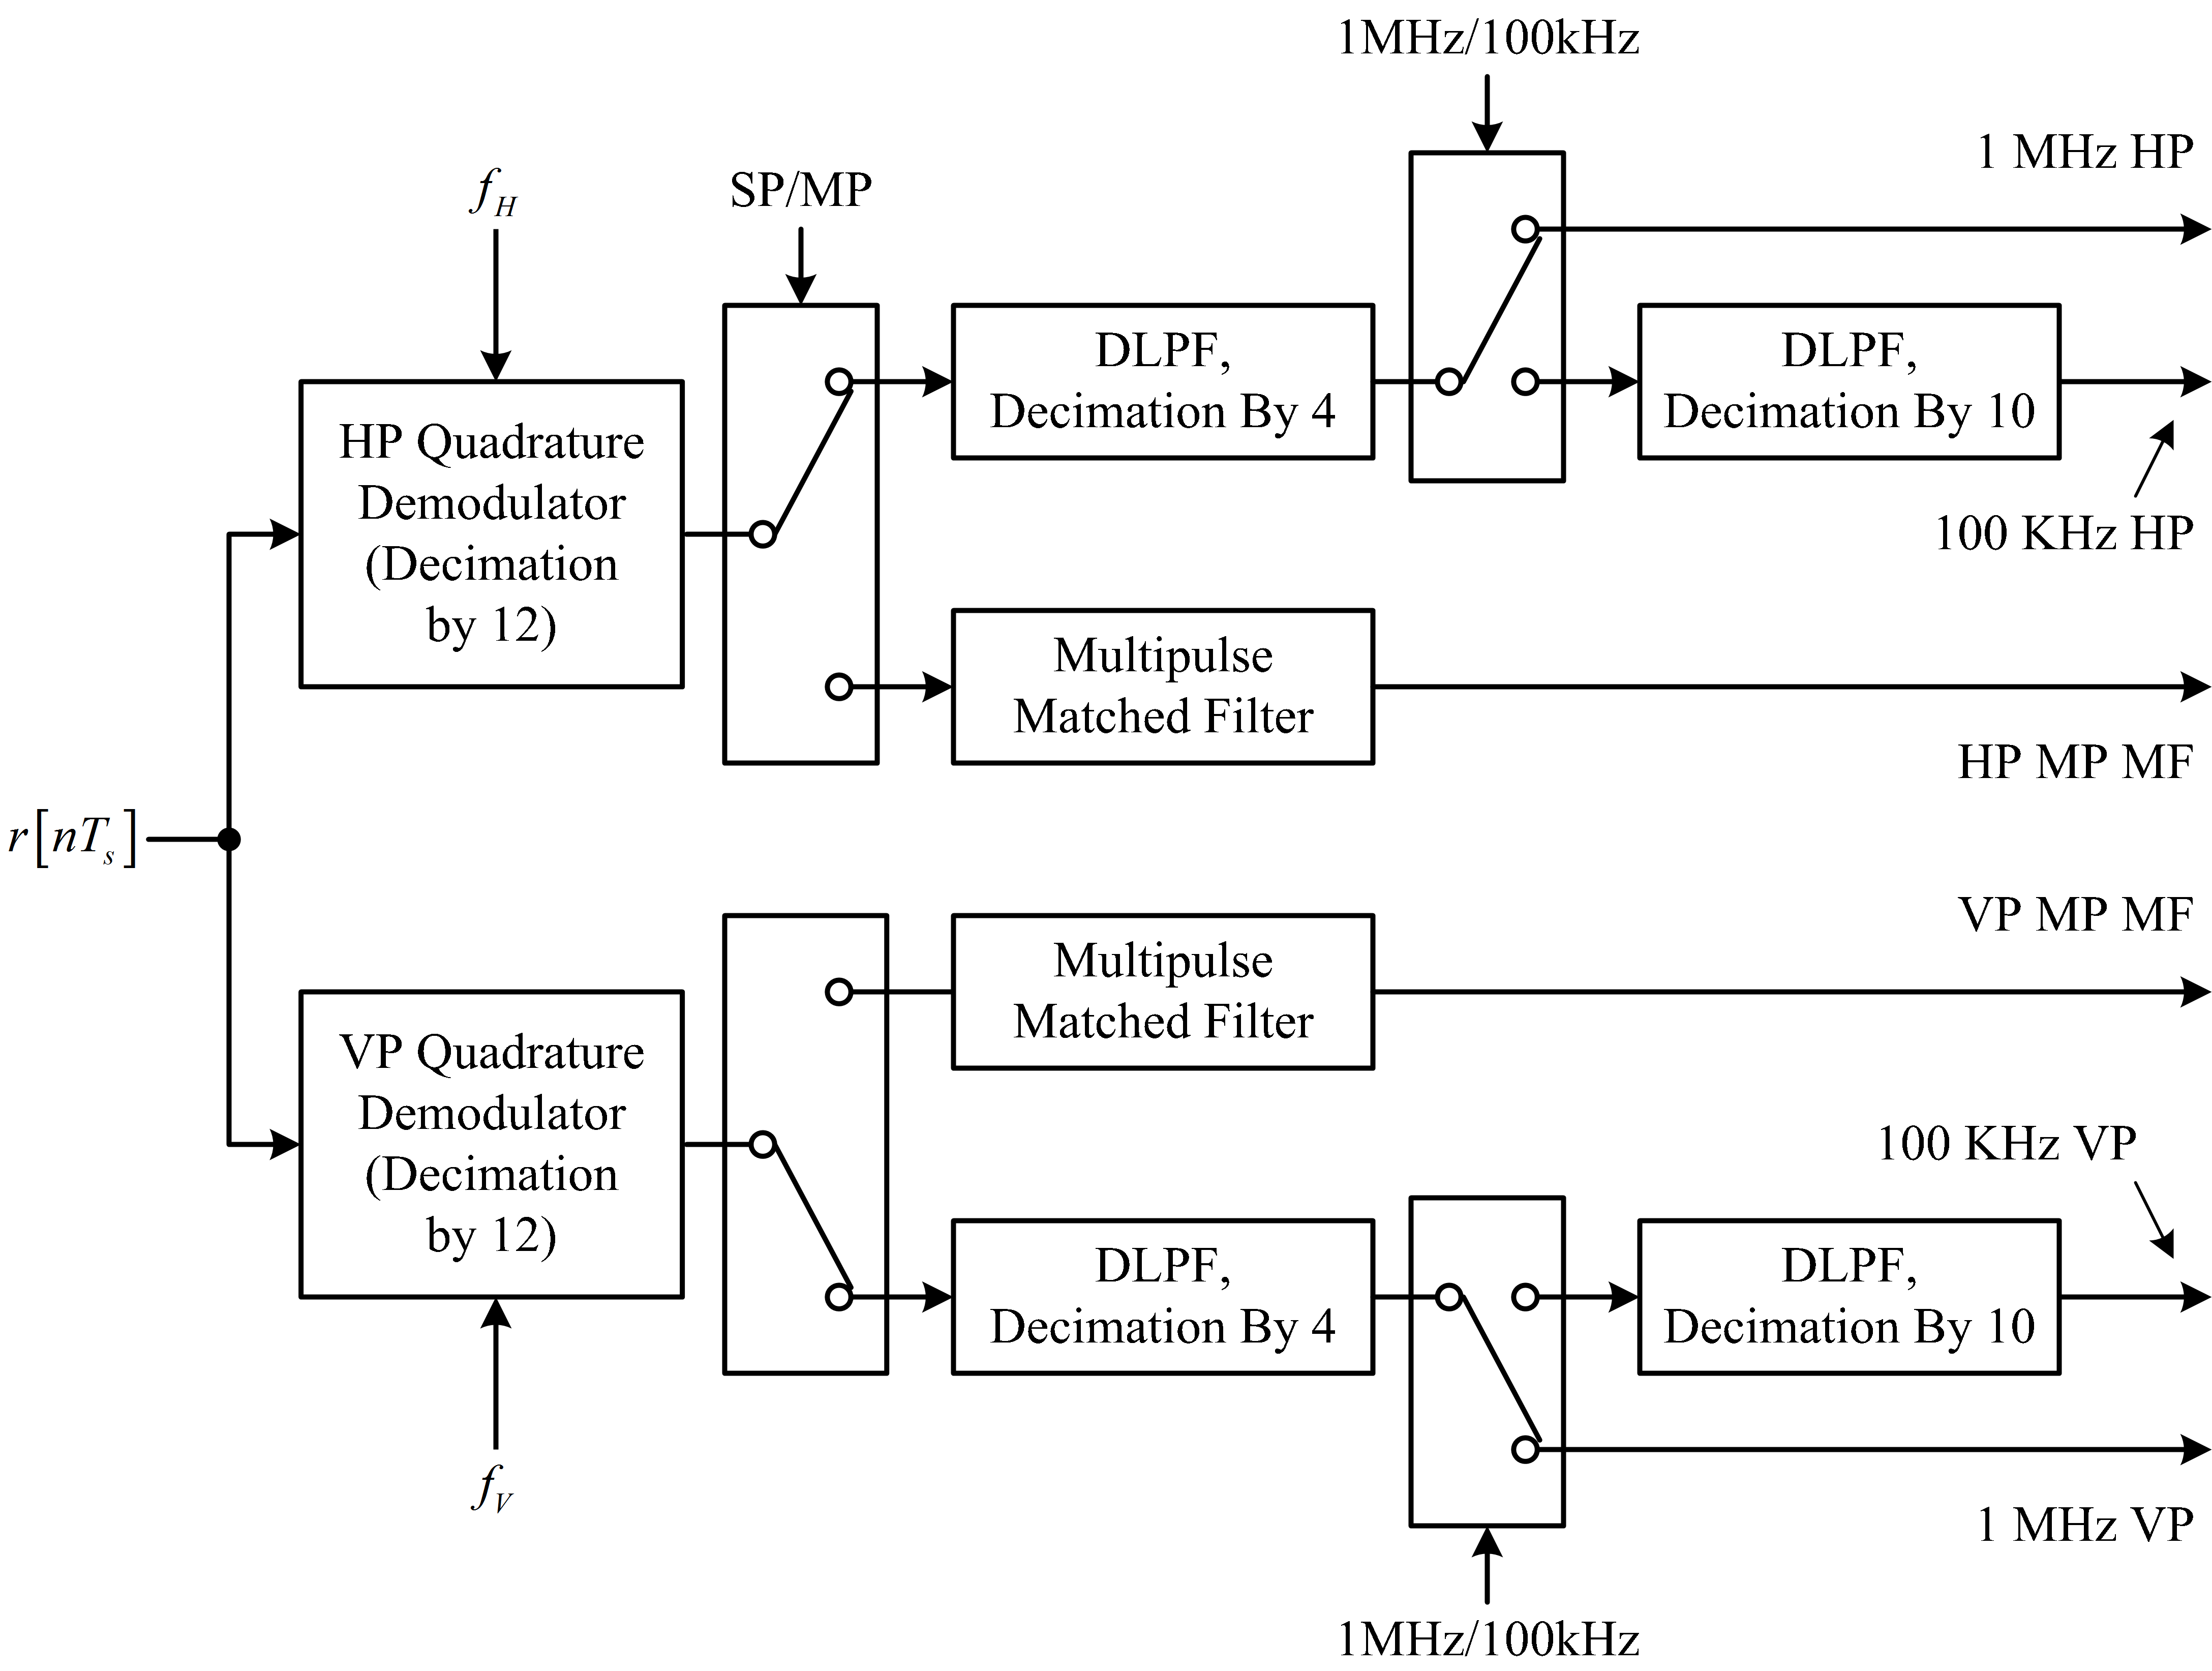
\includegraphics{TbrsDdcTopLevel.png}\medskip{}
  \caption{TBRS Digital Down Conversion}
  \label{fig:TbrsDdcTopLevel}
  \par \end{centering}
\end{sidewaysfigure}

The simulated IF samples are read from the data file generated by
\texttt{TbrsIfSim.py} and input to the quadrature demodulator and
decimation by 12 block. A detailed diagram of this block is shown in
Figure~\vref{fig:QuadratureDemodulator}. This is done for all 11 CSPU
waveforms.

The input samples are split into two paths and multiplied by the
cosine and sine local oscillators (LOs). These LOs ``mix'' the input
sequence to baseband. The frequency of the LOs is equal to the HP IF
frequency (20.5 MHz) plus the estimated target Doppler frequency. The
TBRS generates these LOs using a numerically controlled oscillator
(NCO) VHDL module.
\begin{figure}[ht]
  \noindent \begin{centering}
  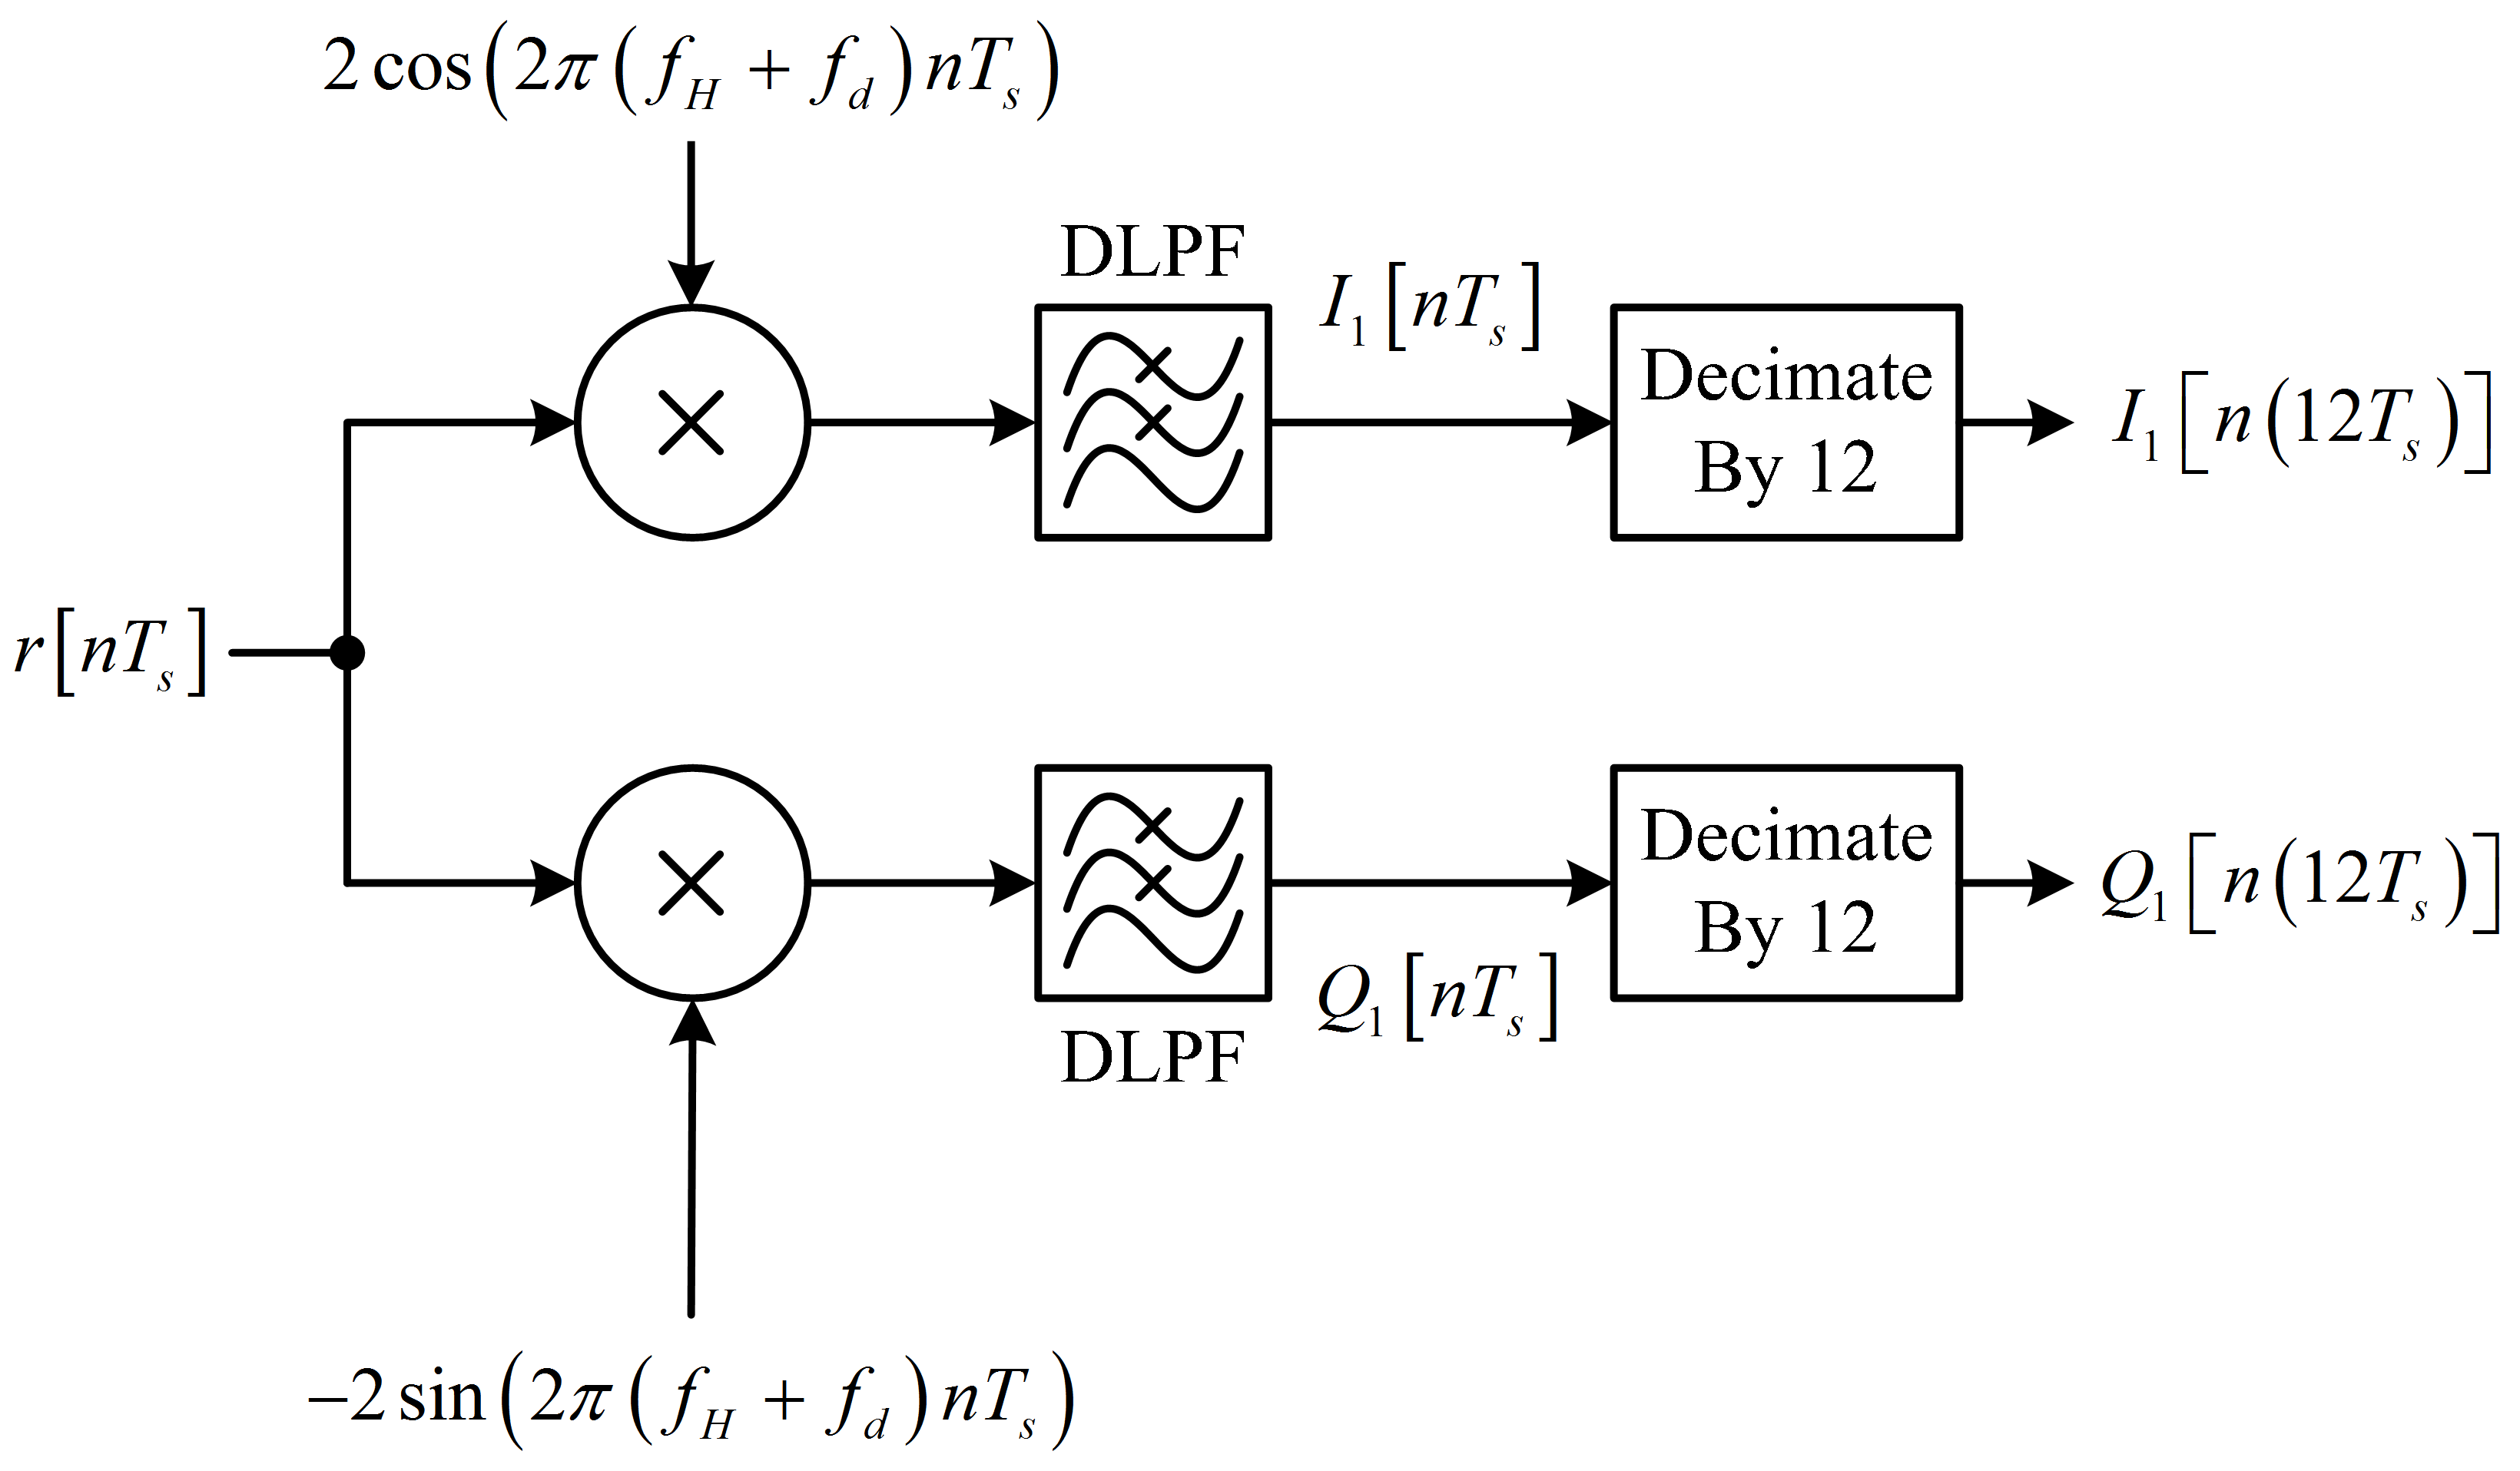
\includegraphics{QuadratureDemodulator.png}\medskip{}
  \caption{Quadrature Demodulator}
  \label{fig:QuadratureDemodulator}
  \par \end{centering}
\end{figure}

The multiplier outputs are fed into DLPFs. These DLPFs are used to
reduce the noise bandwidth by a factor of 12 so that the sampling rate
can be reduced by a factor of 12 (decimated by 12). The simulation
uses the 16-bit integer coefficients used by the TBRS VHDL code to
implement this FIR. The number of coefficients for this filter is 83
and is called an 83-tap FIR.

The sampling rate is reduced from 60 MHz to 5 MHz by the decimation by
12. The processing that follows depends on the CSPU waveform being
simulated. The multiple pulse (MP) waveforms (pulse types 4 and 7) are
processed using the Matched Filter (MF) processing blocks. The single
pulse (SP) waveforms are filtered and decimated by 4 to reduce the
sampling rate from 5 to 1.25 MHz. The DLPF used to decimate by 4 uses
the same 87-tap, 16-bit integer FIR coefficients used by the TBRS
firmware for this filter.

This is the final DDC processing for pulse type 1 and the 1 MHz LFM
pulse types (pulse types 3, 5, 6, 9, and 11). These pulse types all
have a signal bandwidth of 1 MHz. Pulse type 1 is a GCW pulse type
with the 1 MHz bandwidth set by the 1 microsecond pulse width.

The 100 kHz bandwidth pulse types (2, 8, and 10) are filtered again
and their sampling rate is decimated by 10 to 125 kHz. A FIR with 167
taps is used for the filtering. This filter also has 16-bit integer
coefficients.

The MP waveforms are processed in the MF processing blocks. The MF is
a FIR filter with unity coefficients. The number of taps is set equal
to the number of pulse samples $N_p$ across the pulse at the 5 MHz
input sampling rate. This is 125 taps for waveform 4 (25 microsecond
pulse width) and 625 for waveform 7 (125 microsecnd pulse width). The
MF FIR is followed by dual decimators. A block diagram of the waveform
4 MF is shown in Figure~\vref{fig:MultiPulseMF}.

\begin{figure}[ht]
  \noindent \begin{centering}
  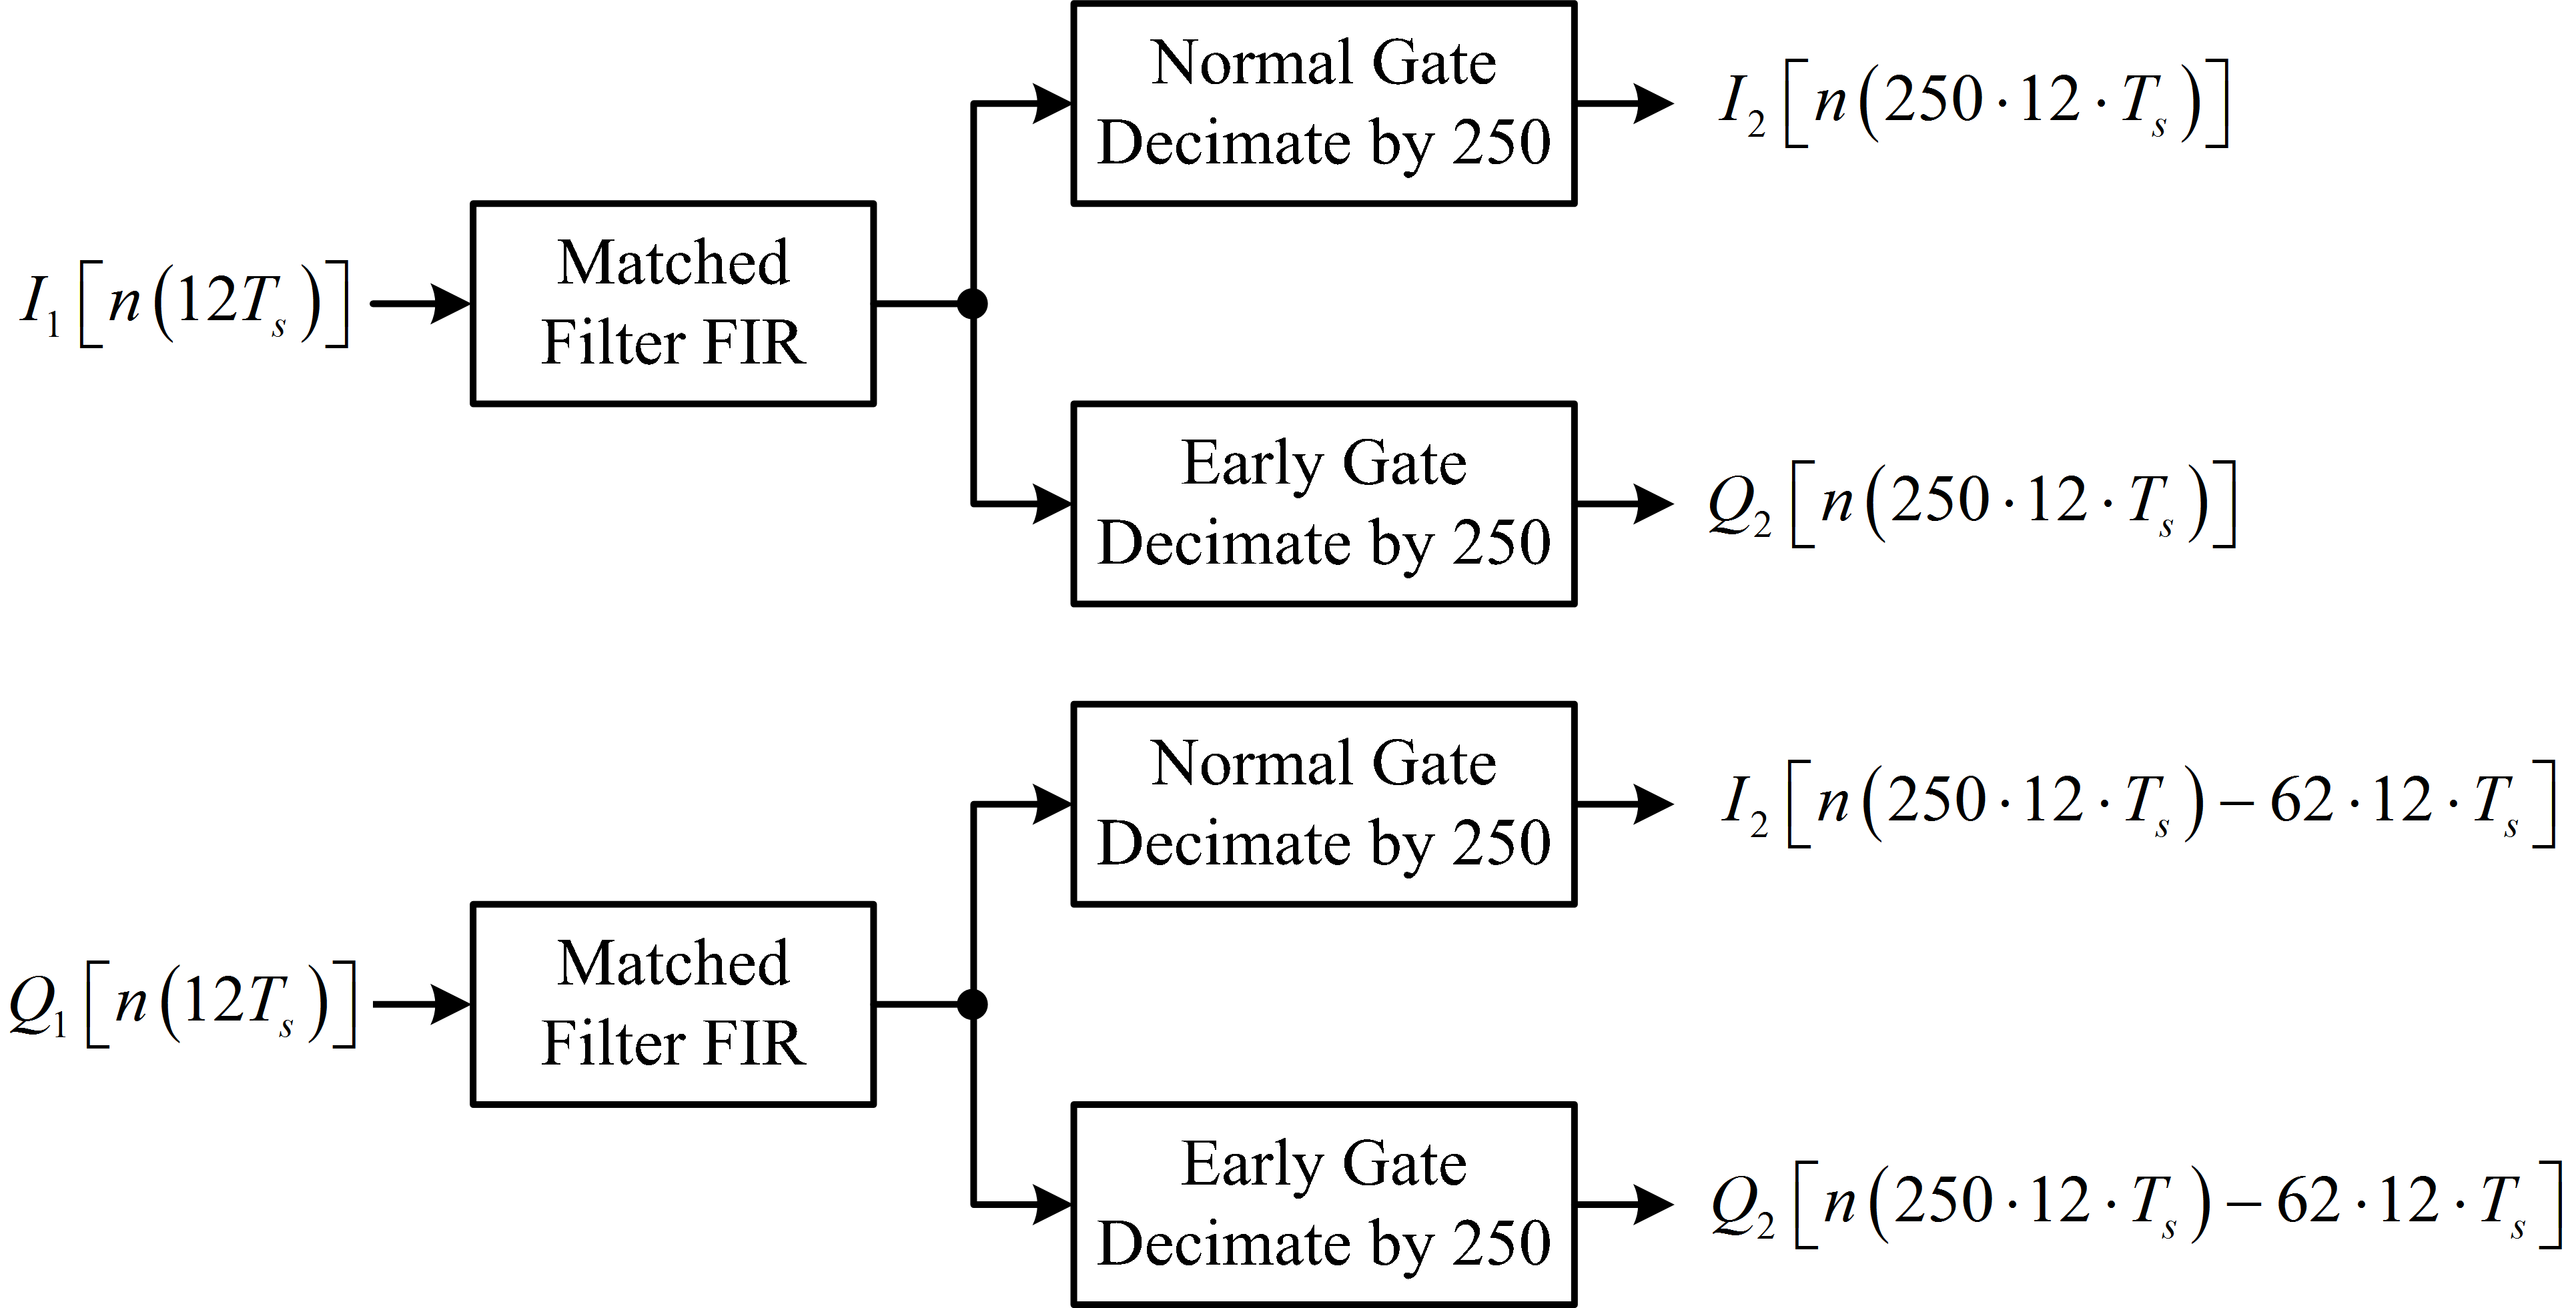
\includegraphics[width=5.0in]{MultiPulseMF.png}\medskip{}
  \caption{Multiple Pulse Matched Filter}
  \label{fig:MultiPulseMF}
  \par \end{centering}
\end{figure}

The dual decimators each decimate by a factor of 250 from 5 MHz to 20
kHz for waveform 4. The ``early gate'' decimator outputs precede the
``normal gate'' outputs by 62 5 MHz samples. For instance, if the a
normal gate decimator output is formed by summing input 5 MHz samples
250 to 499, the corresponding early gate output sample would be formed
by summing input samples 188 to 437.

The dual decimators for waveform 7 are identical except the decimation
factor is 750 instead of 250, and the early gate samples precede the
normal gate samples by 312 5 MHz samples instead of 62.

\texttt{TbrsDdcSim.py} also computes the MF convolution for LFM pulse
types. This is performed in the CSPU system by the digital signal
processing subsystem (DSPS), but is included in
\texttt{TbrsDdcSim.py} for completeness.

A block diagram of the processing is shown in Figure~\vref{fig:LfmMF}
for the 1 MHz LFM waveforms. The input sampling rate is 1.25 MHz. The
impulse response samples $h_i$ and $h_q$ are just the complex
conjugate of the ideal LFM pulse samples. The impulse samples are
multiplied by Taylor range sidelobe reduction weights $w_{sl}$ and
zero-padded to the power of 2 fast Fourier Transform (FFT) size that
will be used to perform the convolution in the frequency domain.
\begin{figure}[ht]
  \noindent \begin{centering}
  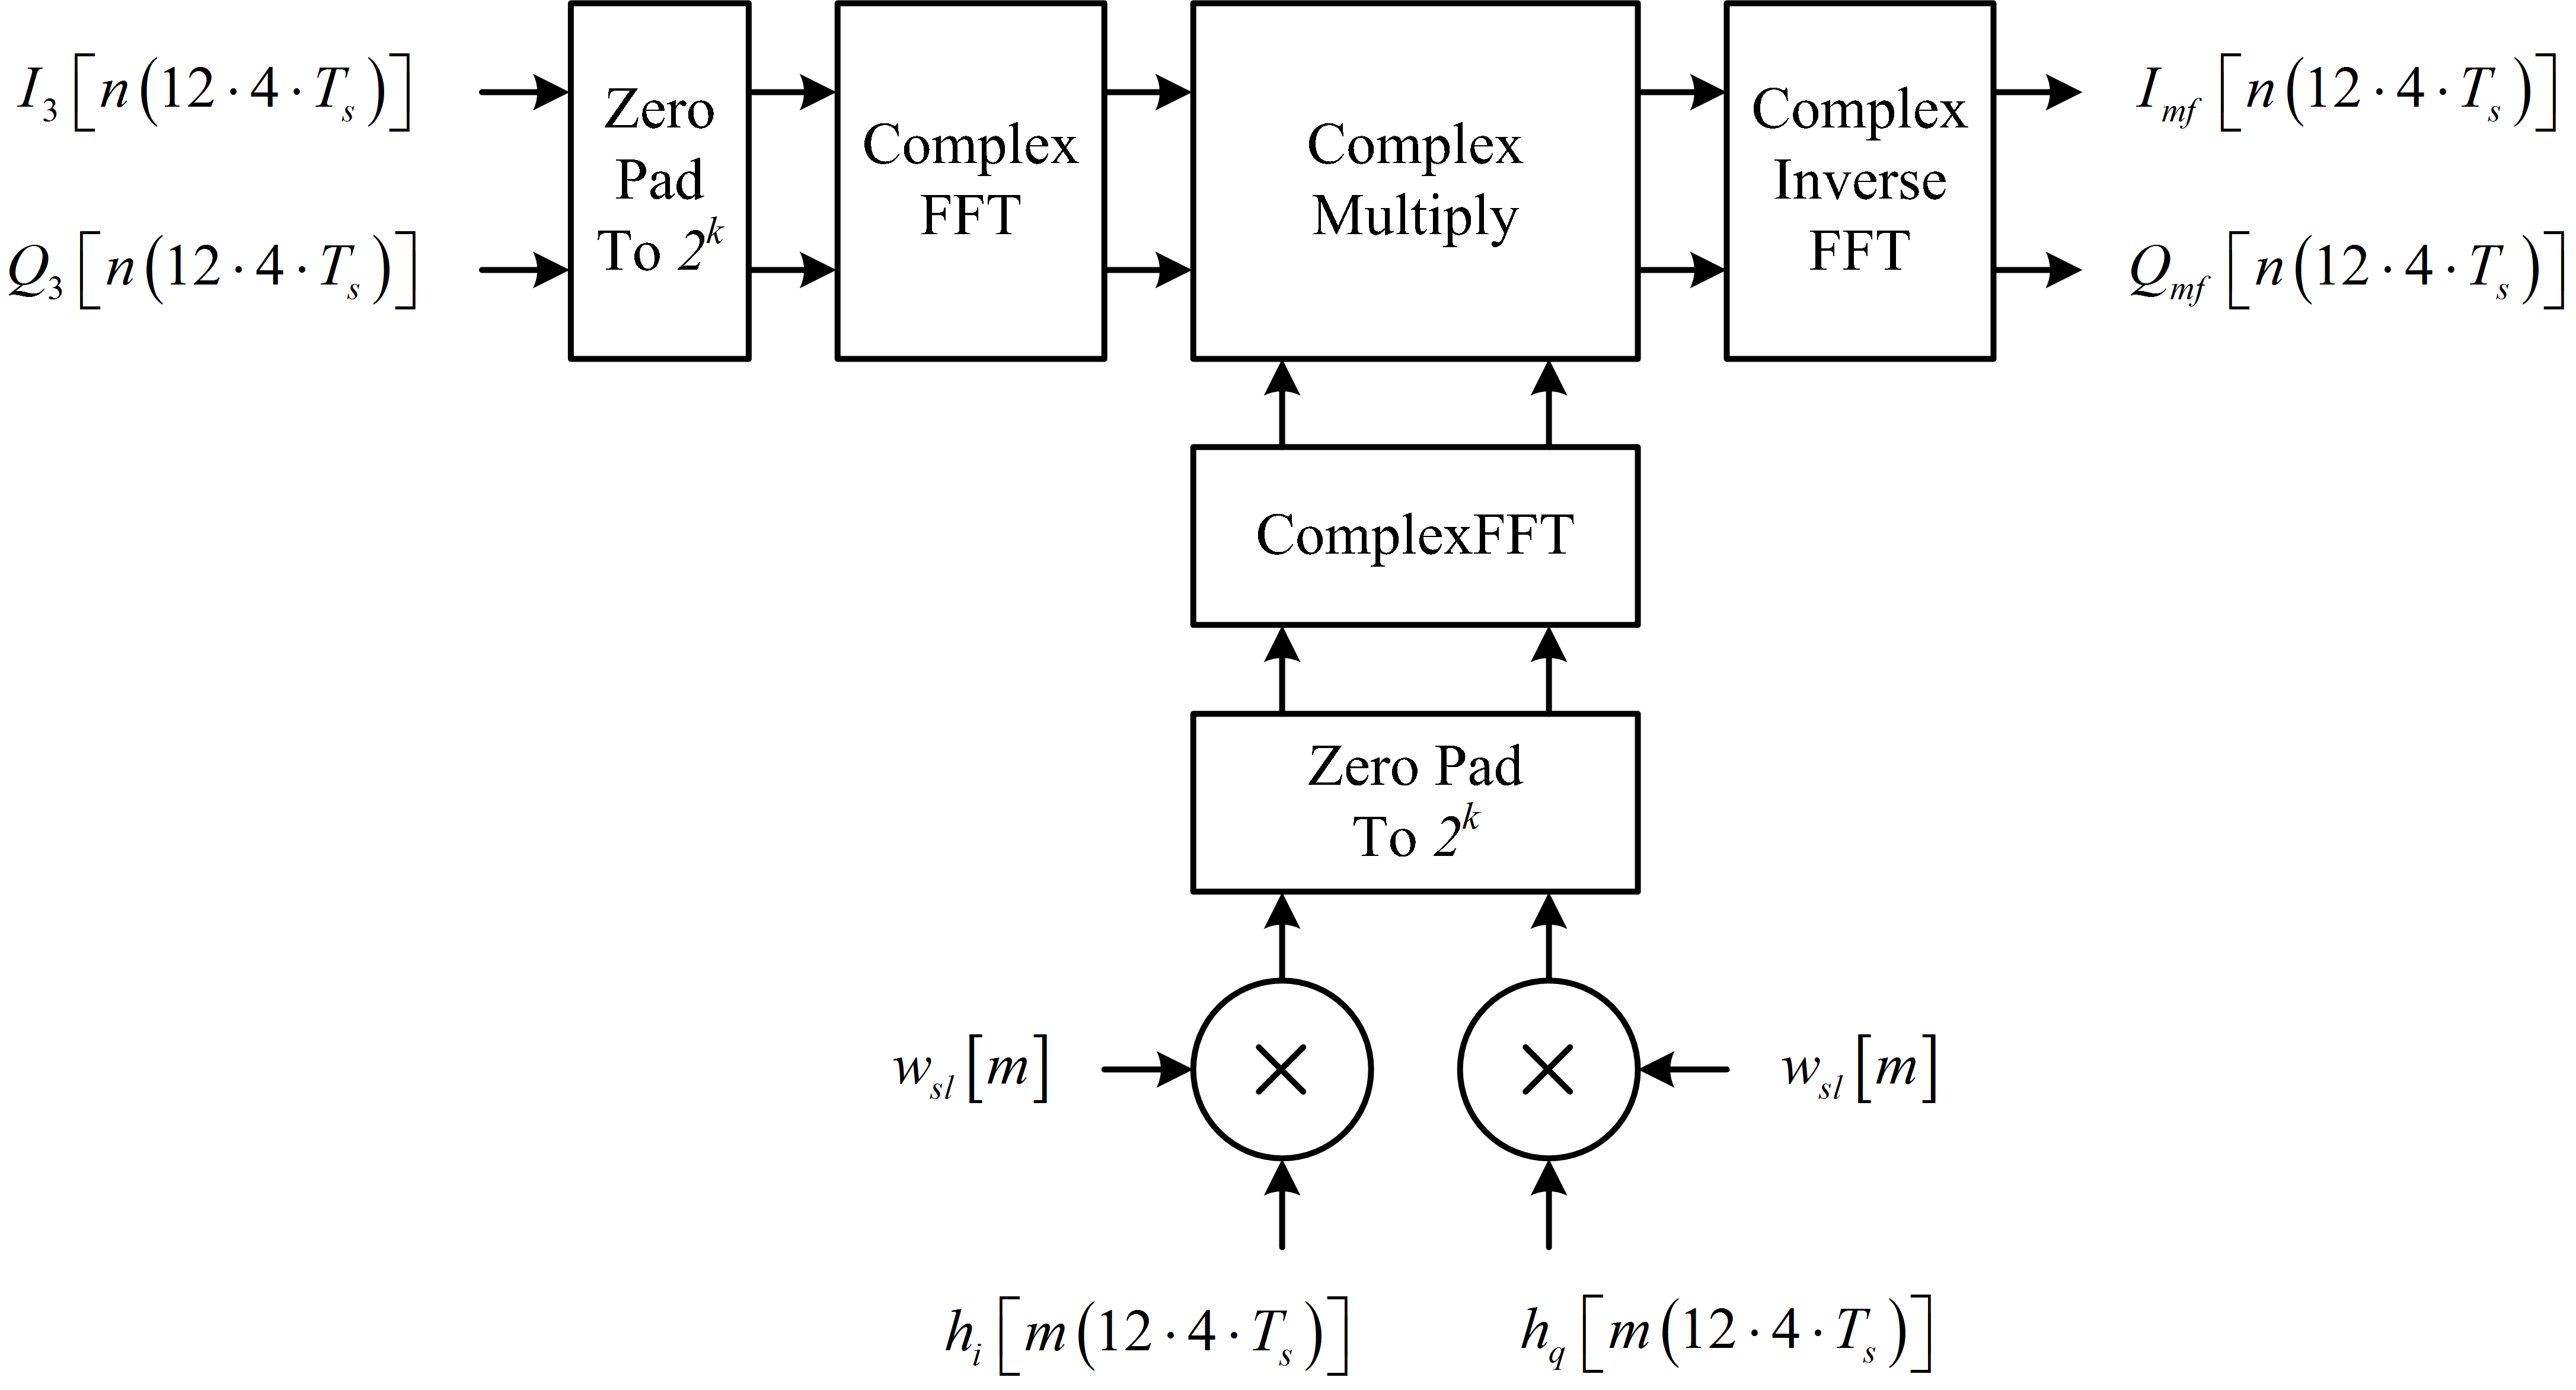
\includegraphics[width=5.0in]{LfmMF.png}\medskip{}
  \caption{LFM Matched Filter}
  \label{fig:LfmMF}
  \par \end{centering}
\end{figure}

The FFT size $N_{fft}$ is determined by the number of baseband ``range window''
samples at the output of the TBRS DDC decimation by 4 $\lp N_{rw}
\rp$ and the number of pulse samples $N_p$. The FFT size is given as
the smallest power of 2 $\lp 2^k \rp$ such that $2^k \ge \lp N_p + N_{rw}\rp$.

The TBRS samples and the weighted impulse response sampes are
zero-padded to $N_{fft}$ and FFT'd. The FFT outputs are point-by-point
vector multiplied and the product is inverse FFT'd to generate the
time domain MF output.

\subsection{Executing the Simulation}

The simulation main source file is named \texttt{TbrsDdcSim.py} as
mentioned above and requires the following additional files:
\begin{itemize}

\item \texttt{fir.py}. This file implements the FIR software objects
for the DLPFs in the DDC.

\item \texttt{util.py}. This file contains utility functions used by
\texttt{TbrsDdcSim.py}.

\item \texttt{lpf1.csv}. This file contains the 83-tap decimation by 12
integer coefficients.

\item \texttt{lpf2.csv}. This file contains the 87-tap decimation by 4
integer coefficients.

\item \texttt{lpf3.csv}. This file contains the 167-tap decimation by 10
integer coefficients.

\item \texttt{IFdata}. This is the folder containing the simulated
``.dat'' and ``.txt'' files generated by \texttt{TbrsIfSim.py}.

\end{itemize}

\texttt{TbrsDdcSim.py} should be located in the same folder as
\texttt{TbrsIfSim.py} and is executed the same way. Again, it is
recommended to run the program from a command prompt.

When \texttt{TbrsDdcSim.py} executes it displays a dialog box that
prompts the user to select the pulse type to process (see
Figure~\vref{fig:TbrsDdcSimSC01}).
\begin{figure}[ht]
  \noindent \begin{centering}
  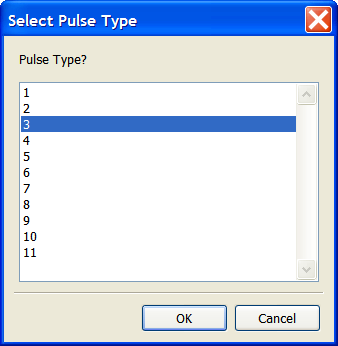
\includegraphics{TbrsDdcSimSC01.png}\medskip{}
  \caption{Input Pulse Type Selection Dialog}
  \label{fig:TbrsDdcSimSC01}
  \par \end{centering}
\end{figure}

The \texttt{IFdata} folder is then searched for ``.dat'' files of the
selected pulse type. If pulse type 3 is selected as shown, files
ending in the pattern ``PT03.dat'' are selected and presented in a
dialog box so the user can select the specific file to process. This
is shown in Figure~\vref{fig:TbrsDdcSimSC02}
\begin{figure}[ht]
  \noindent \begin{centering}
  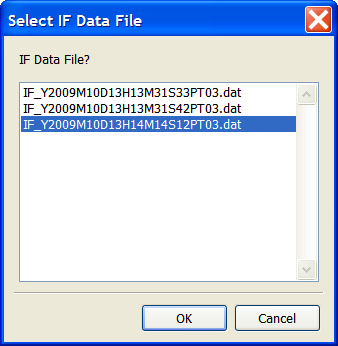
\includegraphics{TbrsDdcSimSC02.png}\medskip{}
  \caption{IF Data File Selection Dialog}
  \label{fig:TbrsDdcSimSC02}
  \par \end{centering}
\end{figure}

If no files for the selected pulse type are located the program exits
and prints an error message to the command line.

If an appropriate file is selected the program then prompts the user
whether to save plot files (see Figure~\vref{fig:TbrsDdcSimSC03}).
\begin{figure}[ht]
  \noindent \begin{centering}
  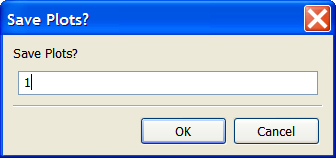
\includegraphics{TbrsDdcSimSC03.png}\medskip{}
  \caption{Save Plot Files Selection Dialog}
  \label{fig:TbrsDdcSimSC03}
  \par \end{centering}
\end{figure}
Simulation plots are generated and displayed to the screen regardless
of the selection. If the user slects to save plot files, they are
saved in the \texttt{plots} sub-folder.

Figure~\vref{fig:TbrsDdcSimSC04} shows the status information printed
to the console window after \texttt{TbrsDdcSim.py} completes
execution.
\begin{figure}[ht]
  \noindent \begin{centering}
  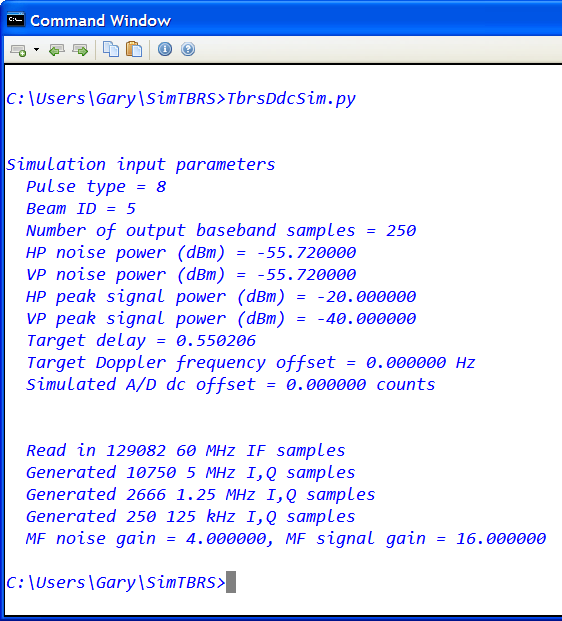
\includegraphics{TbrsDdcSimSC04.png}\medskip{}
  \caption{Console Window Status Information}
  \label{fig:TbrsDdcSimSC04}
  \par \end{centering}
\end{figure}

\texttt{TbrsDdcSim.py} writes output data files to the following
sub-folders:
\begin{itemize}

\item \texttt{5Mdata}. The 5 MHz samples at the output of the
quadrature demodulator and decimation by 12 processing are written to
this folder.

\item \texttt{1\_25Mdata}. The 1.25 MHz samples after decimation by 4
are written to this folder.

\item \texttt{125kdata}. The 125 kHz samples after decimation by 10
are written to this folder.

\item \texttt{plots}. Time domain and spectral plots are written to
this folder.

% To-do. Need to add folders to write out the multi-pulse samples and MF samples.

\end{itemize}

\clearpage
\pagebreak{}

\texttt{TbrsDdcSim.py} generates time domain and frequency domain
spectral plots at the output of each stage of processing. Example
plots are included here for pulse type 8 (128 microsecond pulse width,
100 kHz LFM bandwidth).

The input parameters used to generate the IF data are:
\scriptsize
\begin{verbatim}
pulseType          =            8  # CSPU pulse type.
beamID             =            5  # NOVEM antenna beam number (1..10)
numBasebandSamples =          250  # Number of output baseband samples to generate.
Pn_H               =   -55.720000  # HP noise power (dBm).
Pn_V               =   -55.720000  # VP noise power (dBm).
Ps_H               =   -20.000000  # HP peak signal power (dBm).
Ps_V               =   -40.000000  # VP peak signal power (dBm).
tau_d              =     0.550206  # Target delay (fraction of 60 MHz IF sample window).
f_d                =     0.000000  # Target Doppler frequency offset (Hz).
muIF               =     0.000000  # Simulated A/D dc offset (counts).
\end{verbatim}
\normalsize

The calculated signal and noise counts are:
\scriptsize
\begin{verbatim}
A_H                =   259.053786  # HP Amplitude (counts).
A_V                =    25.905379  # VP Amplitude (counts).
sigma_H            =     2.998299  # HP Sigma (counts).
sigma_V            =     2.998299  # VP Sigma (counts).
\end{verbatim}
\normalsize

The following plots were generated when processing the IF data file:
\begin{itemize}

\item Figure~\vref{fig:5MHzTimeDomainPT8_AH0_AV0M2}. These are the I
and Q time domain 5 MHz sample plots for both HP and VP.

\item Figure~\vref{fig:IQSpectrumPT8_AH0_AV0M2}. These are HP and VP
spectral plots of the 5 MHz samples.

\item Figure~\vref{fig:1_25MHzTimeDomainPT8_AH0_AV0M2}. These are the I
and Q time domain 1.25 MHz sample plots after decimation by 4.

\item Figure~\vref{fig:1_25MHzSpectrumPT8_AH0_AV0M2}. These are HP and VP
spectral plots of the 1.25 MHz samples.

\item Figure~\vref{fig:125kHzTimeDomainPT8_AH0_AV0M2}. These are the I
and Q time domain 125 kHz sample plots after decimation by 10.

\item Figure~\vref{fig:125kHzSpectrumPT8_AH0_AV0M2}. These are HP and VP
spectral plots of the 125 kHz samples.

\item Figure~\vref{fig:125kHzMatchedFilterPT8_AH0_AV0M2}. These are the I
and Q time domain MF sample plots.

\item Figure~\vref{fig:125kHzMfLogMagPT8_AH0_AV0M2}. These are the log
magnitude time domain MF sample plots.

\end{itemize}


\begin{figure}[ht]
  \noindent \begin{centering}
  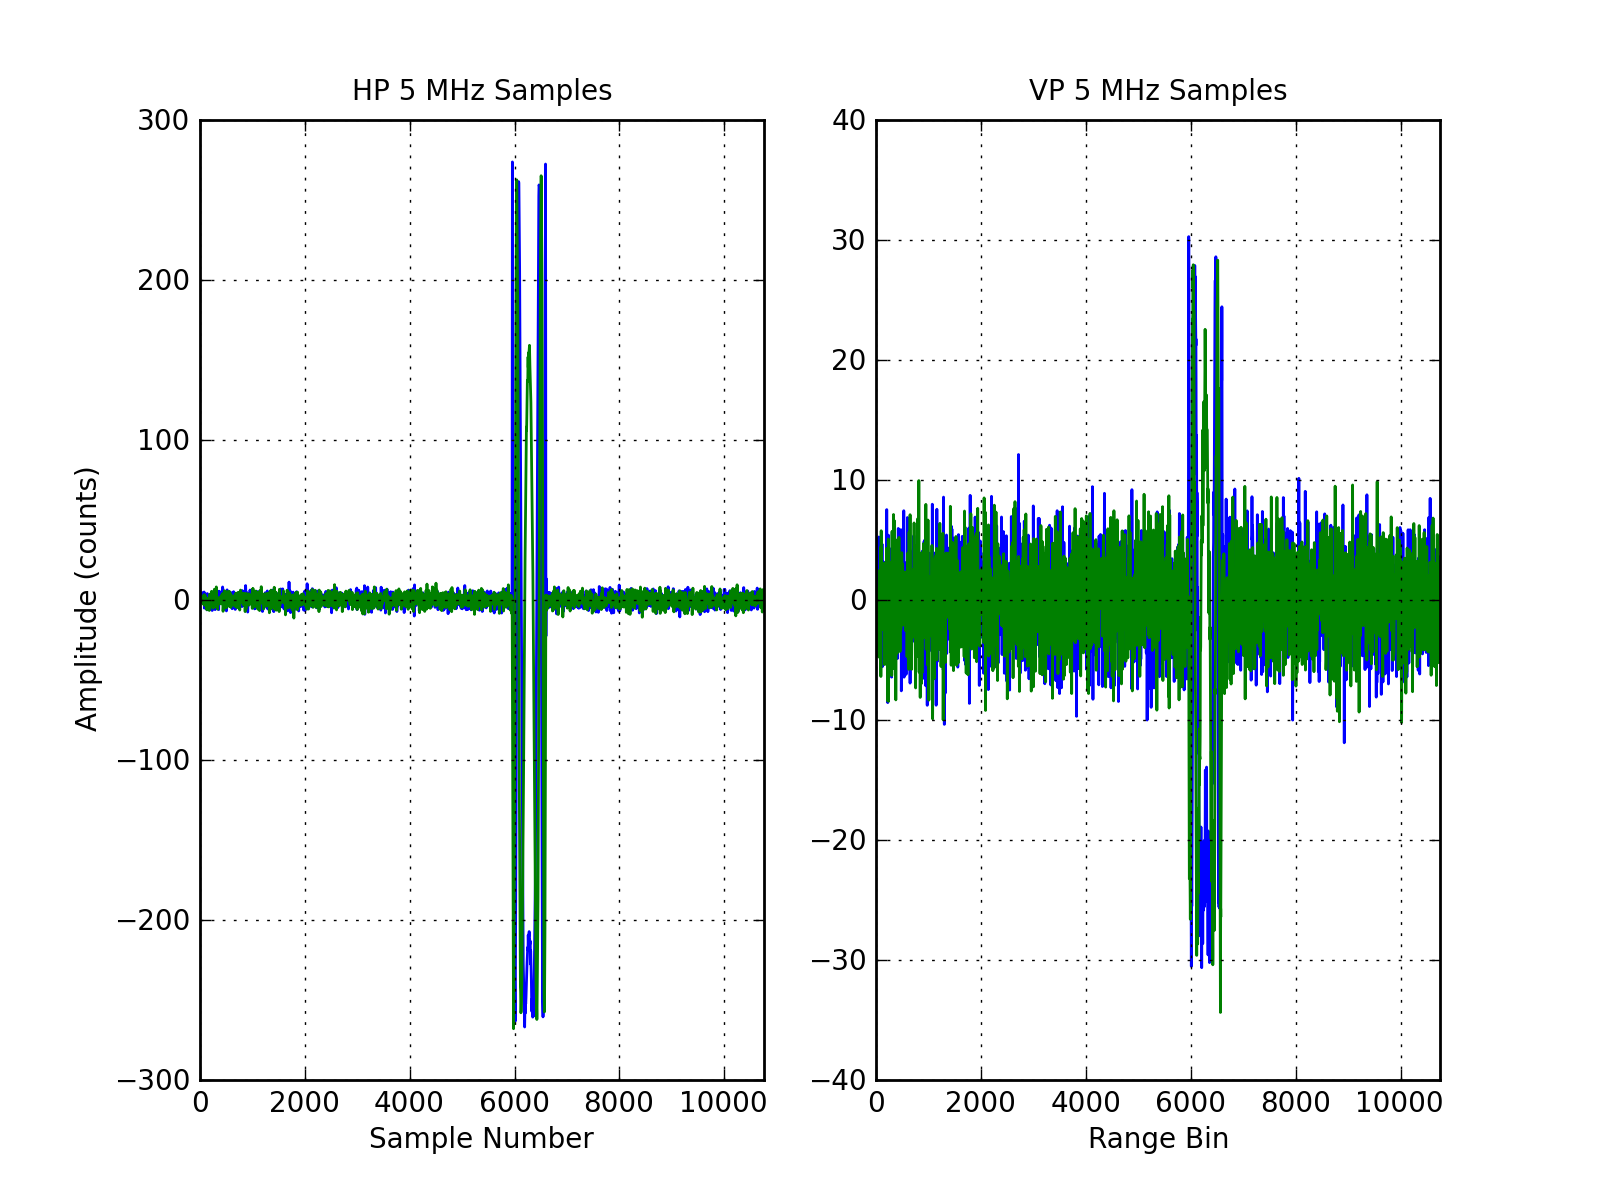
\includegraphics[width=4.75in]{5MHzTimeDomainPT8_AH0_AV0M2.png}\medskip{}
  \caption{5 MHz I and Q Time Domain Samples}
  \label{fig:5MHzTimeDomainPT8_AH0_AV0M2}
  \par \end{centering}
\end{figure}

\begin{figure}[htb]
  \noindent \begin{centering}
  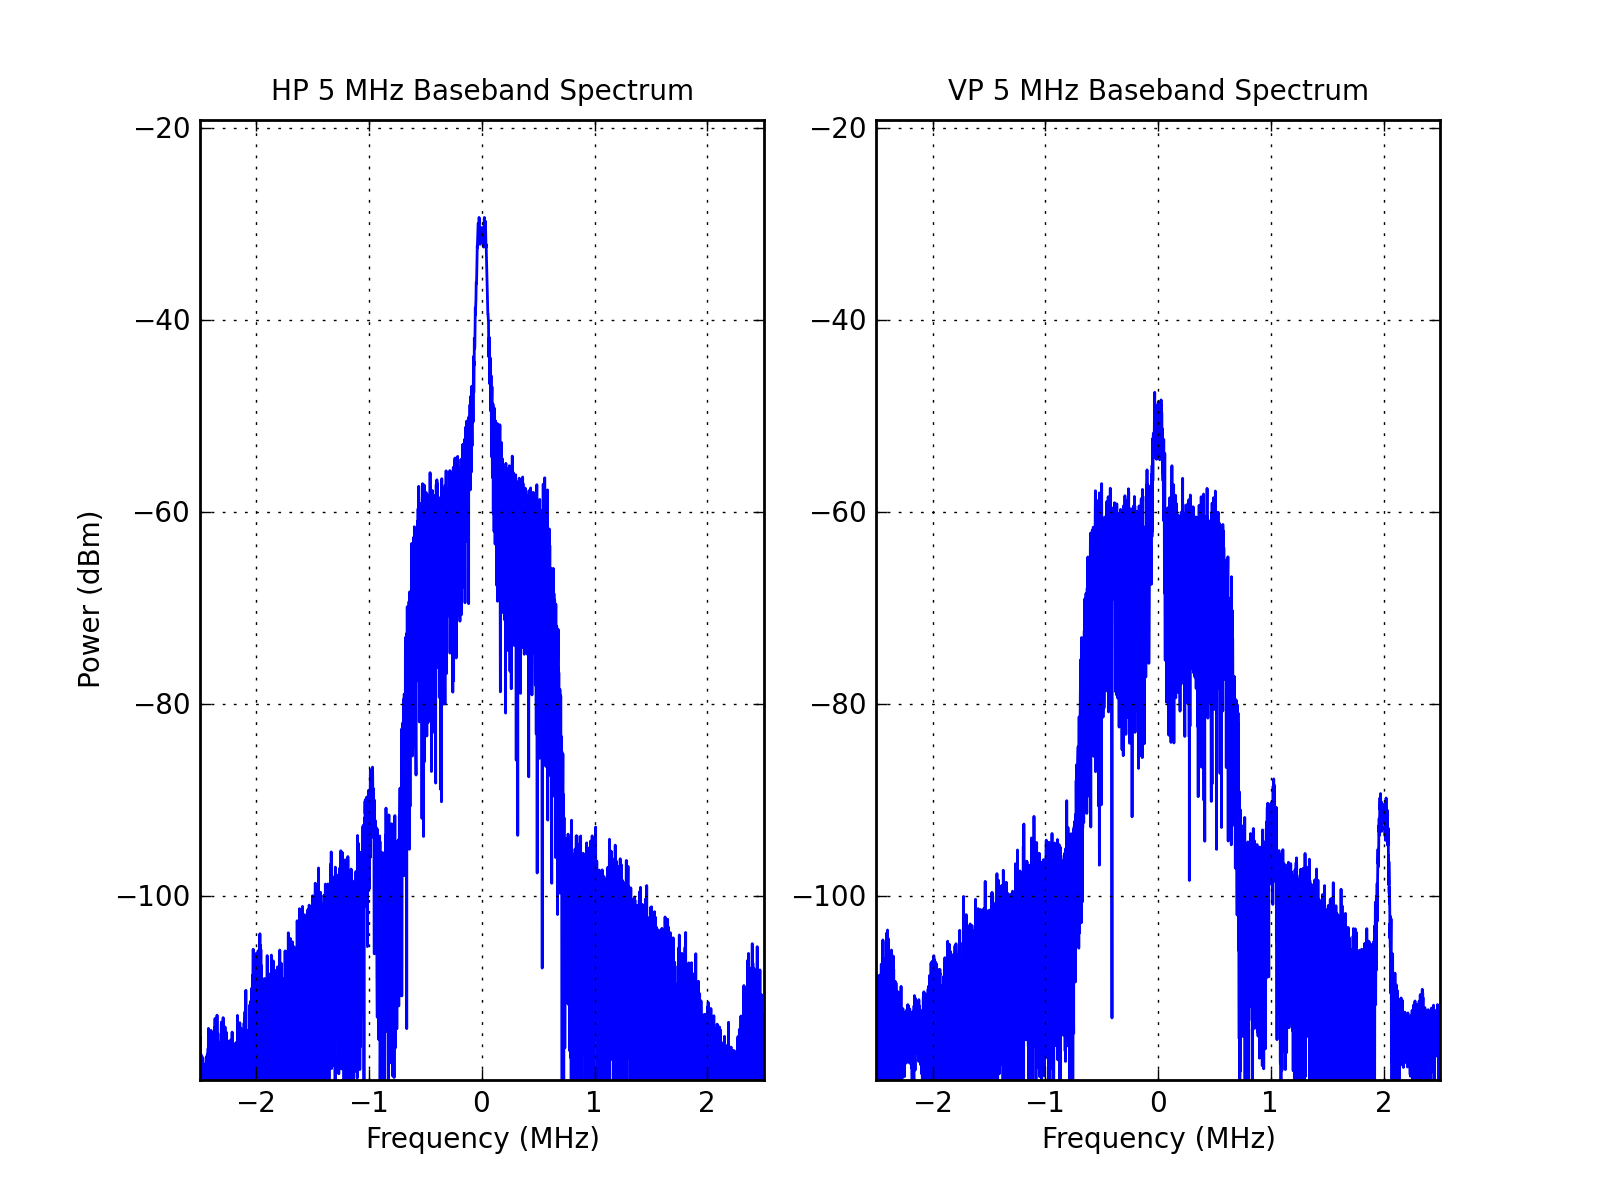
\includegraphics[width=4.75in]{IQSpectrumPT8_AH0_AV0M2.png}\medskip{}
  \caption{5 MHz Spectral Plots}
  \label{fig:IQSpectrumPT8_AH0_AV0M2}
  \par \end{centering}
\end{figure}

\begin{figure}[ht]
  \noindent \begin{centering}
  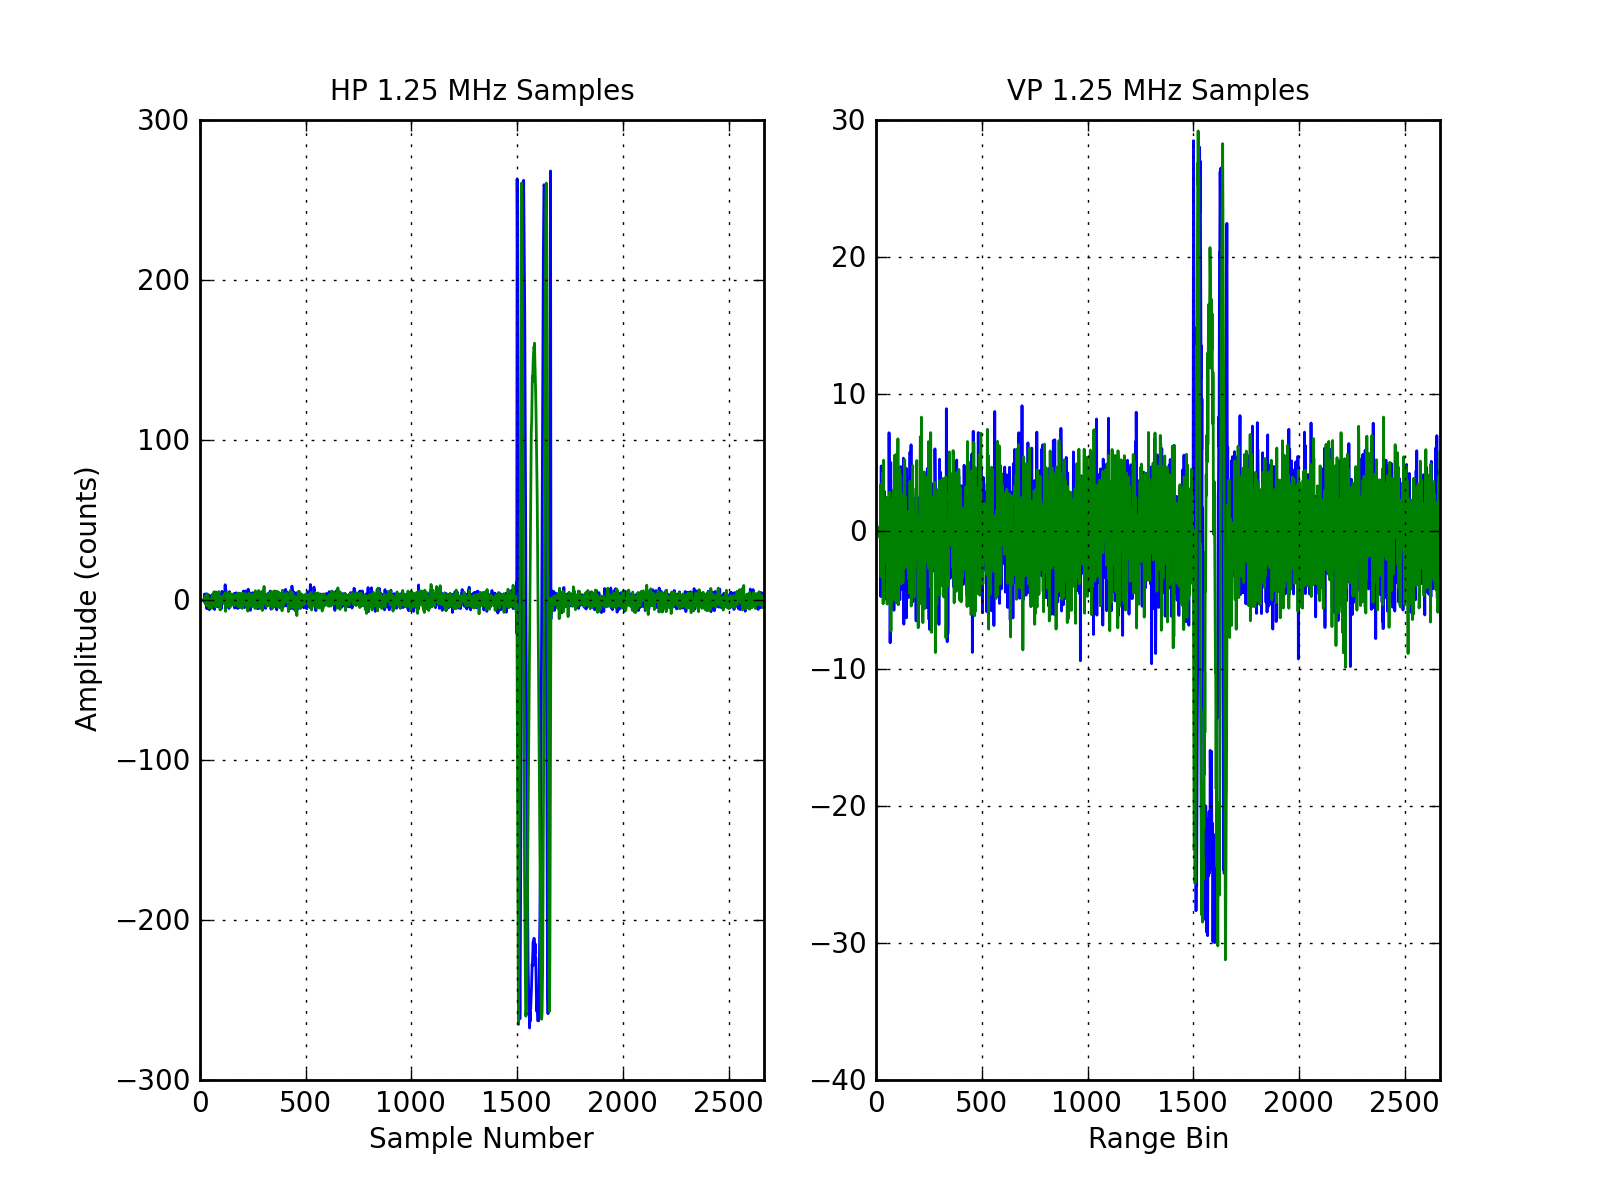
\includegraphics[width=4.75in]{1_25MHzTimeDomainPT8_AH0_AV0M2.png}\medskip{}
  \caption{1.25 MHz I and Q Time Domain Samples}
  \label{fig:1_25MHzTimeDomainPT8_AH0_AV0M2}
  \par \end{centering}
\end{figure}

\begin{figure}[htb]
  \noindent \begin{centering}
  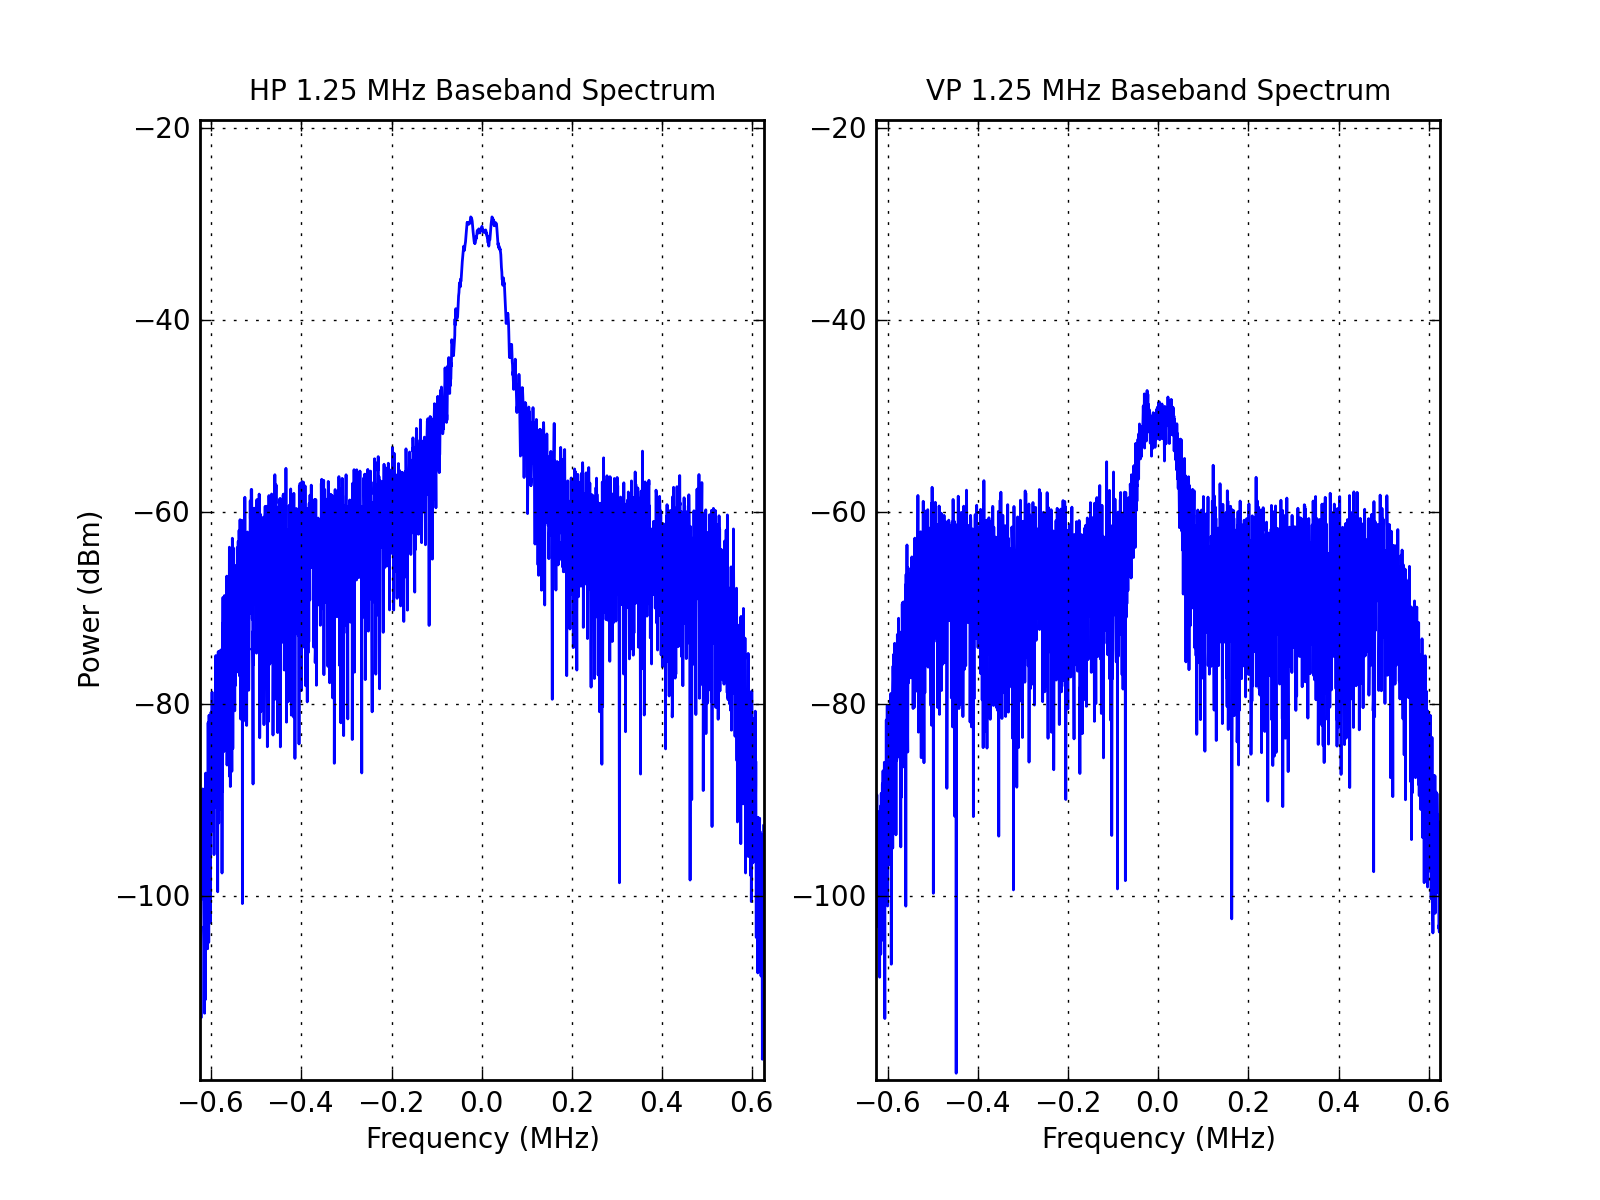
\includegraphics[width=4.75in]{1_25MHzSpectrumPT8_AH0_AV0M2.png}\medskip{}
  \caption{1.25 MHz Spectral Plots}
  \label{fig:1_25MHzSpectrumPT8_AH0_AV0M2}
  \par \end{centering}
\end{figure}

\begin{figure}[ht]
  \noindent \begin{centering}
  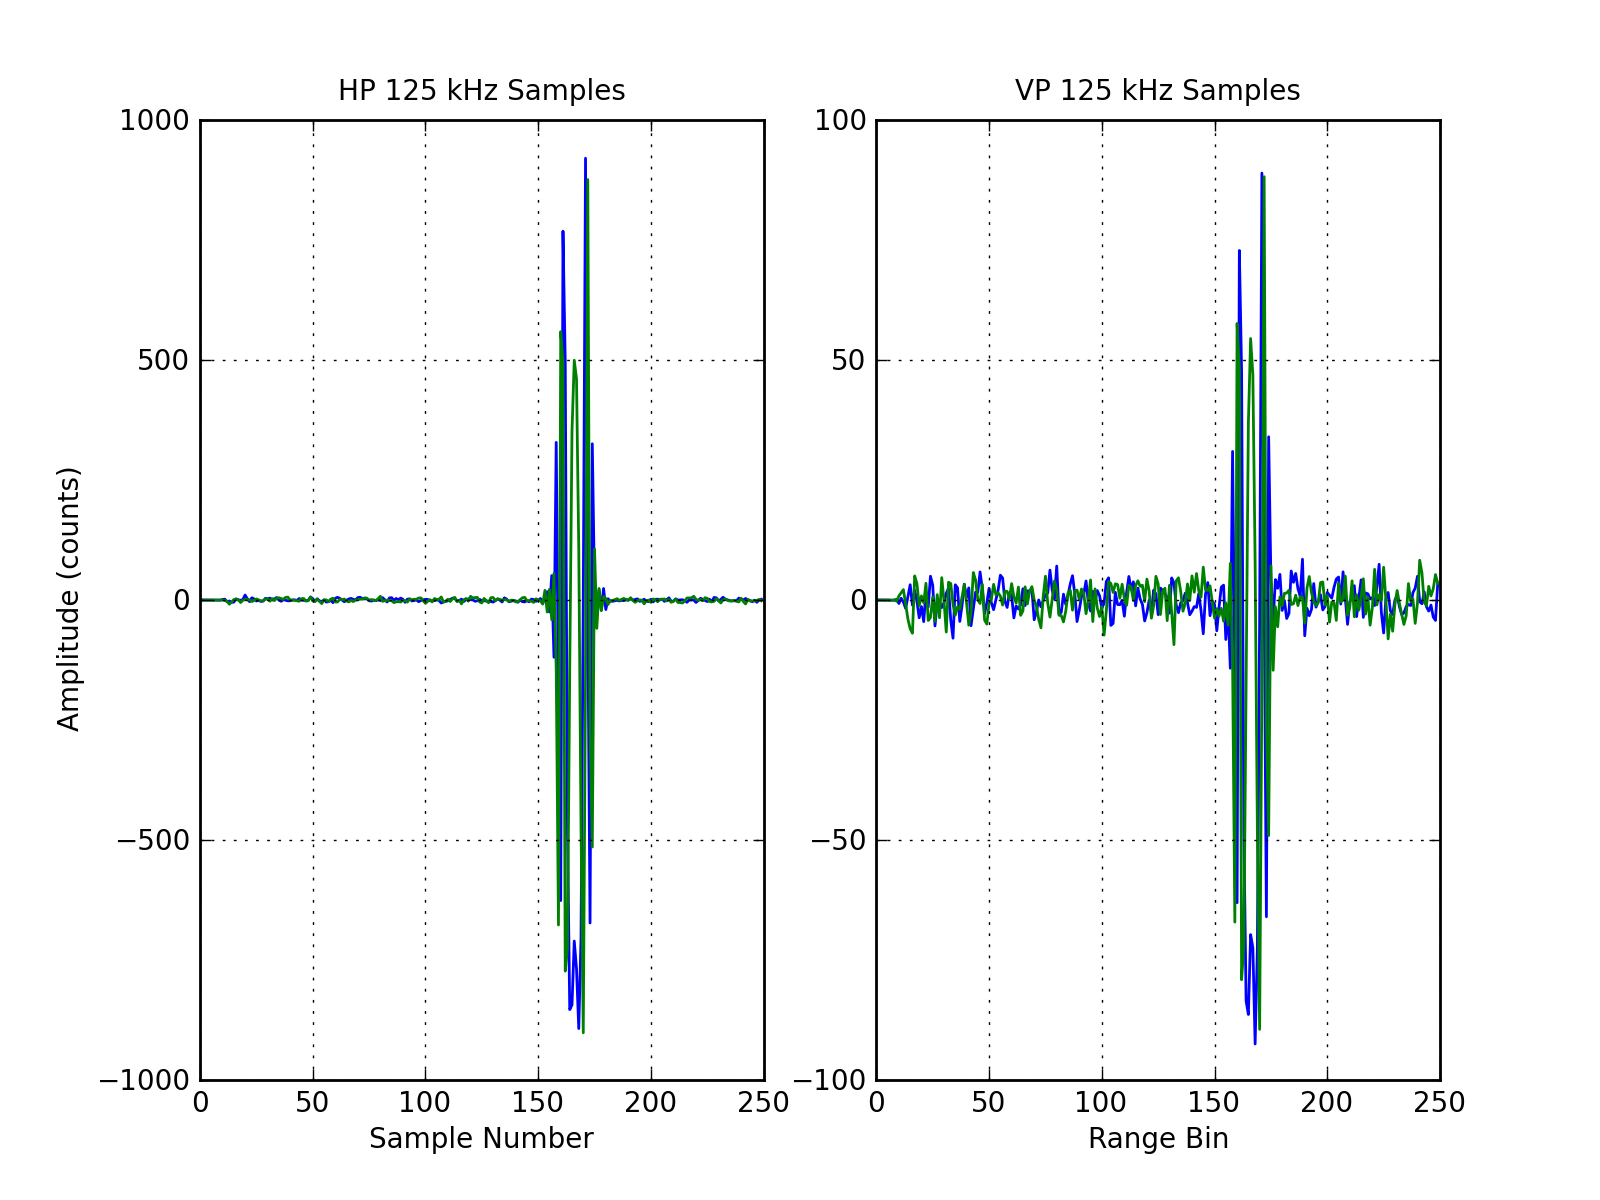
\includegraphics[width=4.75in]{125kHzTimeDomainPT8_AH0_AV0M2.png}\medskip{}
  \caption{125 kHz I and Q Time Domain Samples}
  \label{fig:125kHzTimeDomainPT8_AH0_AV0M2}
  \par \end{centering}
\end{figure}

\begin{figure}[htb]
  \noindent \begin{centering}
  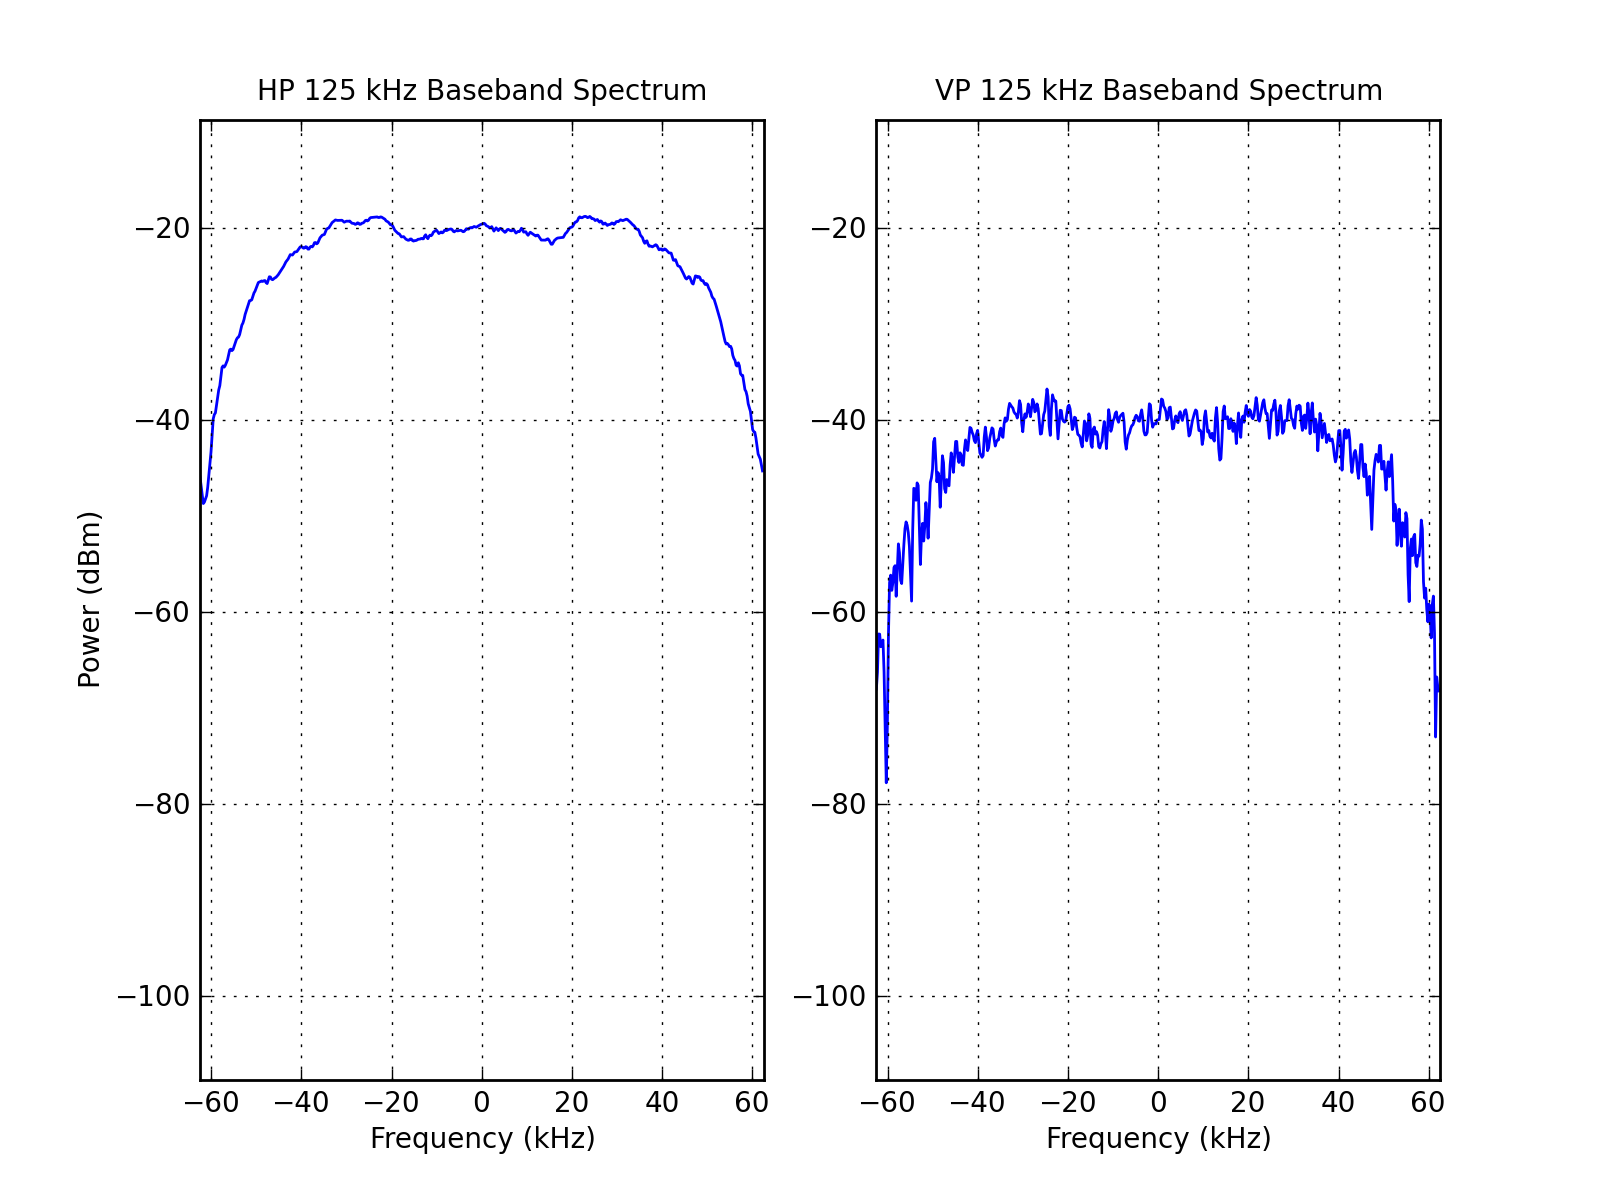
\includegraphics[width=4.75in]{125kHzSpectrumPT8_AH0_AV0M2.png}\medskip{}
  \caption{125 kHz Spectral Plots}
  \label{fig:125kHzSpectrumPT8_AH0_AV0M2}
  \par \end{centering}
\end{figure}

\begin{figure}[ht]
  \noindent \begin{centering}
  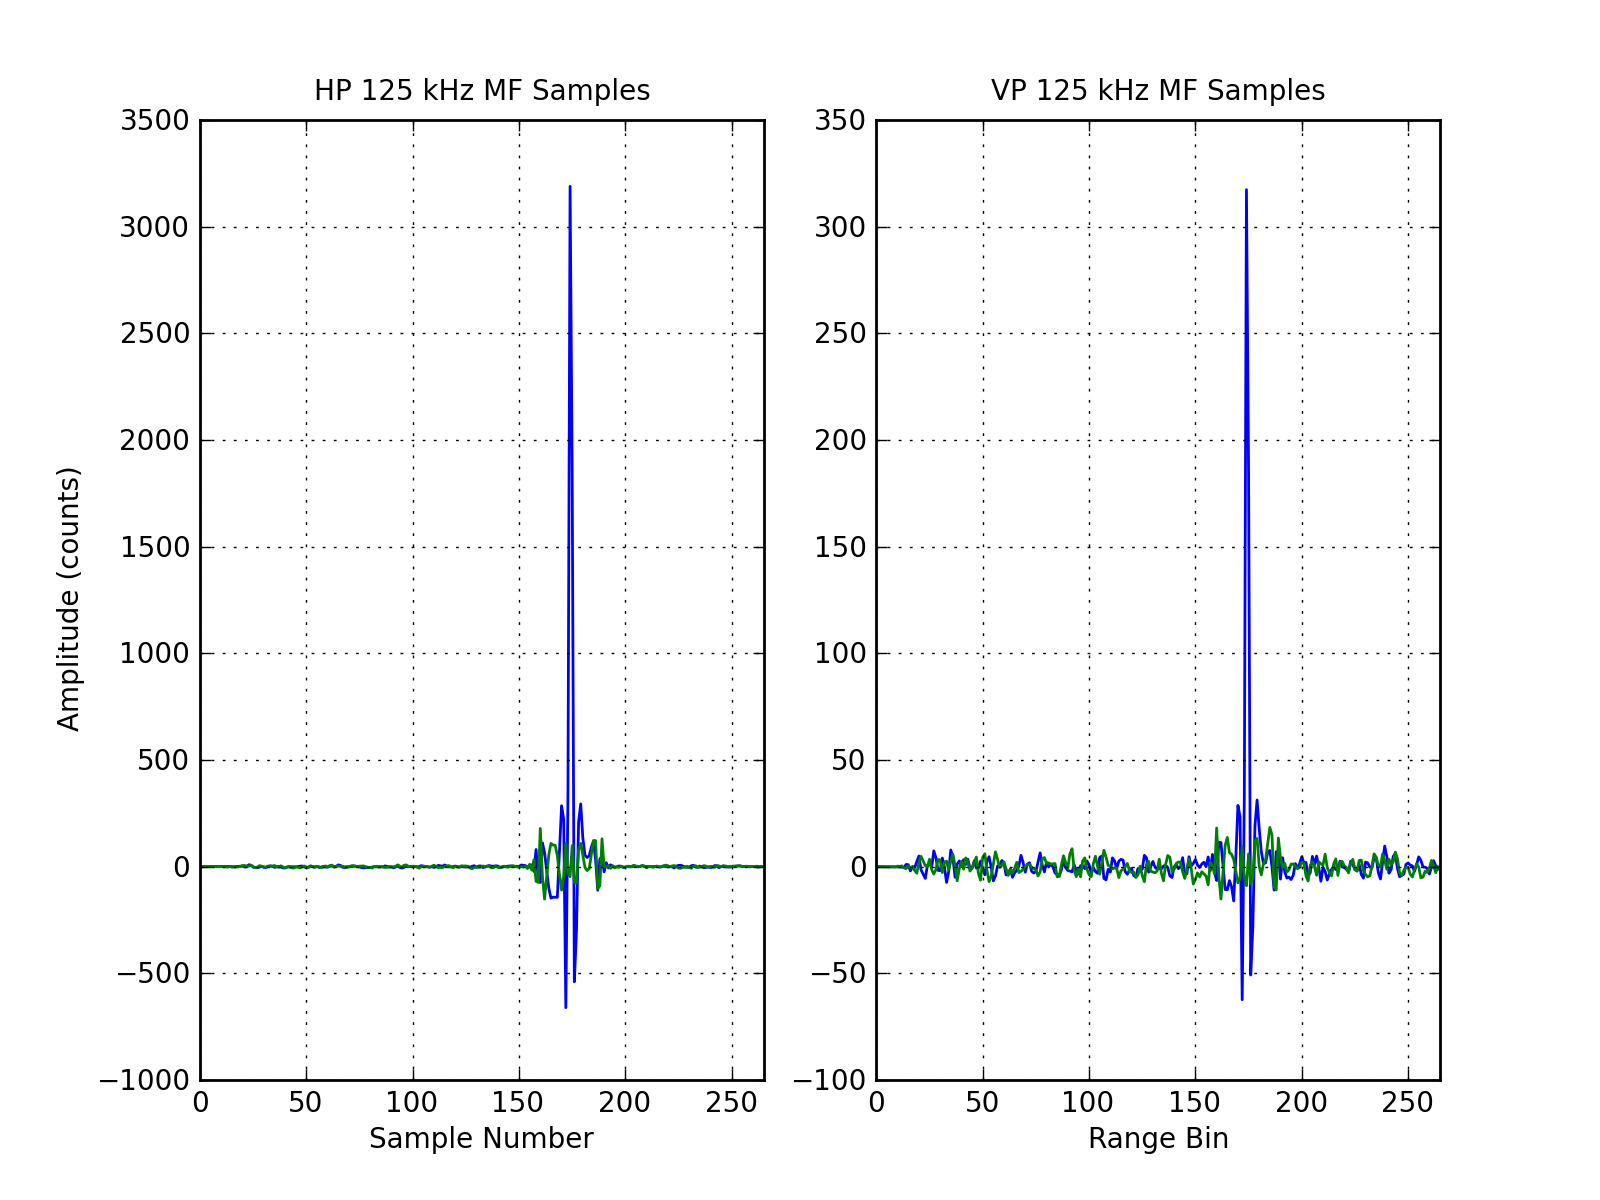
\includegraphics[width=4.75in]{125kHzMatchedFilterPT8_AH0_AV0M2.png}\medskip{}
  \caption{Matched Filter I and Q Time Domain Samples}
  \label{fig:125kHzMatchedFilterPT8_AH0_AV0M2}
  \par \end{centering}
\end{figure}

\begin{figure}[htb]
  \noindent \begin{centering}
  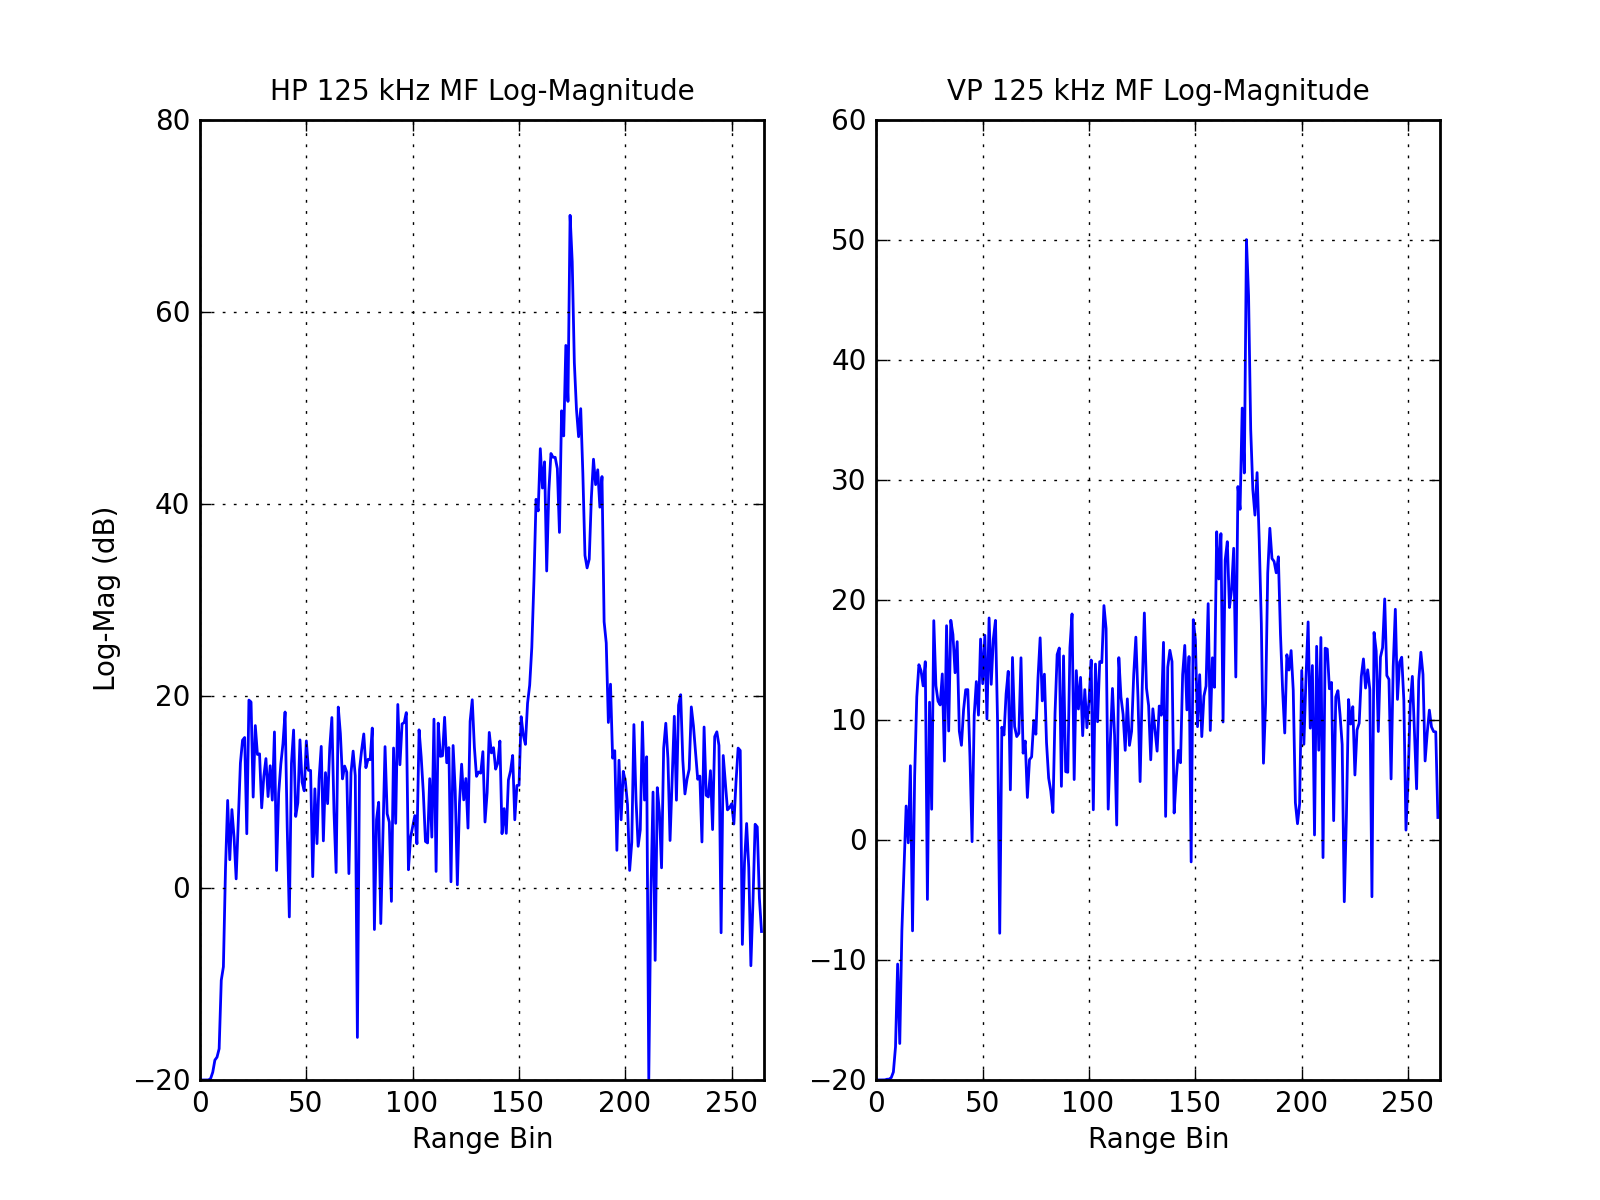
\includegraphics[width=4.75in]{125kHzMfLogMagPT8_AH0_AV0M2.png}\medskip{}
  \caption{Matched Filter Log Magnitude Time Domain Samples}
  \label{fig:125kHzMfLogMagPT8_AH0_AV0M2}
  \par \end{centering}
\end{figure}


\end{document}
